\documentclass[10pt,a4paper]{article}
%\documentclass[10pt,a4paper]{beamer}
\usepackage[utf8]{inputenc}
\usepackage{amsmath}
\usepackage{amsfonts}
\usepackage{amssymb}
\usepackage{graphicx}
\usepackage{subfigure}
\usepackage[left=2cm,right=2cm,top=2cm,bottom=2cm]{geometry}
\usepackage{kpfonts}
\usepackage[numbers]{natbib}
%other options include: round, curly, angle, or default options

\usepackage{media9}

\author{Zhixuan Cao}%\\ Advisor: Abani Patra}
\title{Computing of Volcanic Plume with Mesh-free Method}

\begin{document}

\maketitle
%\tableofcontents
\section{Abstract}
Smoothed particle hydrodynamics(SPH) has several advantages over mesh-based methods in modeling multiple phase free boundary flows. We develop a new volcano plume model employing two phases fluid dynamics governing equations, three-dimensional coordinates, SPH method and message passing interface (MPI) standard parallel computing. $SPH-\varepsilon$ turbulence model is adopted to capture sub-particle scale turbulent entrainment. Corrected formulism of SPH is used to handle tensile instability and deficiency of particle distribution near the boundaries. The model is first verified by a JPUE simulation where velocity and concentration distribution along axis and acrross cross section are compared with experiments.Then a typical volcano plume is simulated with this model. Top height of the plume and profiles of several local variables are compared with previous simulation results of existing plume models. Analysis on the plume evolution process also shows that the plume near the vent maintains a concentric structure with an inner dense core surrounded by an outer shear margin which is consistent with previous simulation.
\section{Introduction}
%\subsection{Explosive eruption and associated hazards}
%Plume usually forms in a explosive eruption.
The dynamics of explosive eruption clouds has been the central issue of volcanology science for a long time.
%\citep{bullard1962volcanoes, woods1988fluid, valentine1989numerical}.
Primary hazards associated with explosive “grey volcanoes” include pyroclastic density currents (flows and surges), the widespread deposition of airfall tephra, and the threats posed by volcanic ash. In addition, there are also other secondary hazards associated with volcanoes\citep{lockwood2013volcanoes}.
Simulation of all possible hazzards with one model is difficult due to diversity among these hazzards. Our concerns in current work is the risks that volcanic ash posesed on aircrafts and communities. During volcanic eruptions, volcanic ash transport and dispersion models (VATDs) are used to forecast the location and movement of ash clouds over hours to days. Those VATDs models use input parameters, called “eruption source parameters”, such as plume height $H$, mass eruption rate $\dot{M}$, duration $D$, and the mass fraction distribution of erupted debris finer than about $4 \Phi$ (or $63  \mu m$), which can remain in the cloud for many hours or days. Observational data on the value of such parameters are usually unavailable in the first minutes or hours after an eruption is detected. Moreover, observed plume height may change during an eruption, requiring rapid assignment of new parameters. Usually, plumes models are used to provide sources terms for VATDs. This paper reports a new 3D volcano plume model target at providing more accurate source parameters for VATDs.\\
%The ash harzards are usually predicted by volcanic ash transport and dispersion models (VATDs) which takes output of a volcano plume model as input. For example, the plume height and physics properties along the plume axis are fisrt predicted by a one dimensional(1D) plume model, such as bent \cite{bursik2001effect}, and the radial ash particle distribution is approximated with a presumed distribution. Then the concentration distribution is taken by VATDs, such as hysplit \cite{stein2015noaa}, as input for ash transportation and dispersion prediction. The accuracy of plume model is crucial for ash dispersion simulation. We target at developing new plume model that will provide more accurate source term for VATDs.\\ 
%Several volcano plume models adopting mesh-based methods have been developed in the past few decades. SPH (smoothed particle hydrodynamics), a mesh free method, is applied in various areas including free boundary flow simulation. It has several advantages over mesh-based methods in modeling volcano plume.
The basic physics behind the ascent and collapse of volcanic columns has been understood for more than half a century\citep{morton1956turbulent, settle1978volcanic, wilson1978control}. Several volcano plume models have been developed in the past few decades. Specific aspects of a plume have been studied by one dimensional(1D) plume models which describe the steady state solution of a plume under idealized boundary conditions.
%\subsection{1D Plume Model}
The effects of magma type and vent conditions \citep{woods1988fluid, woods1995decompression}, atmospheric conditions\citep{sparks1997volcanic, woods1993moist, bursik2001effect}, external surface water\citep{koyaguchi1996formation}, thermal disequilibrium, and particle fallout\citep{woods1991particle} have been assessed in increasing details through 1D numerical simulations. In these 1D models, the entrainment of air is evaluated based two coefficients: entrainment coefficient for the verical plume and the entrainment coefficient that describes the effect of wind. Different 1D models adopt different entrainment coefficients based on specific formulation or calibration against well-documented cases studies. The feedback from plume to atmosphere is ignored in 1D models. Even though determination of essential parameters such as the entrainment rate are not based on first principles, such simple models nevertheless allow us to investigate the importance of physical mechanisms in a volcanic plume. In addition, these simplified models (eg. \citep{mastin2007user}) requires little computational sources and can run on standard personal computers or on web sites in very short time. As a result, software (\citep{267, 1194, 3541} for volcano plume development, \citep{114, draxler2015hysplit} for ash dispersion and transportation) based on 1D model are still pretty popular. While these 1D models can generate well-matched results with three dimensional(3D) models for weak plumes, much greater variability is observed for strong plume scenarios, especially for local variables\cite{costa2016results}. In addition, the need for greater skills in associated hazards forecasts with 1D models requires 2D and 3D models.\\
The development of two dimensional(2D) and three dimensional(3D), time-dependent, and multiphase numerical models for volcano plume have provided new explanations for many features of explosive volcanism. One of these 3D models is PDAC \citep{neri2003multiparticle}  which is a non-equilibrium, multiphase, 3D compressible flow model. Conservation equations for each phase is solved separately with finite volume method. And a parallel computing version of PDAC was developed recently \cite{ongaro2007parallel}. Advanced numerical techniques(second order scheme and semi-explicit time upgrading) was also adopted to improve the accuracy of PDAC\cite{carcano2013semi}. 
% These studies focused on the unsteady and multiphase features of eruption clouds, and demonstrated some features of eruption clouds, including stable column, column collapse, and oscillating behavior. 
%The resolution of simulation can reach 20m (with a maximum size of 100 meters) on a domain of $12 \times 14 \times 8km$ by making use of the power of paralell computing\citep{neri20074d}, the resolution can reach minimum 20m and maximum 100m. However, their predictions for column collapse were not always quantitatively consistent with those of the steady 1-D models in which the entrainment coefficient based on the laboratory experiments \citep{neri1994influence} was used.\\
Suzuki\citep{suzuki2005numerical} developed a three-dimensional time-dependent fluid dynamics model (which is refered as SK-3D) that can reproduce the entrainment process of eruption clouds with relative simpler physics but higher order of accuracy and high spatial resolution, which is applicable to time-dependent phenomena in actual volcanological situations. SK-3D is able to correctly reproduces the quantitative features of turbulent mixing in and around the JPUE(jet or plume which is ejected from a nozzle into a uniform environment) under the ideal experimental conditions. A serials of simulations based on SK-3D was conducted, including determination of the entrainment coefficient of eruption columns as a function of height\citep{suzuki2010numerical}, study the effect of wind feild on entrainment coefficient\citep{suzuki20133d}, establishment of the relationship between the observable quantities of the eruption clouds and the eruption conditions at the vent (previously, such relationship is based on 1D models and greatly depends on empirical constants)\citep{suzuki2009three}, investigation of the effect of the intensity of turbulence in the umbrella cloud on dispersion and sedimentation of tephra\citep{koyaguchi2009effect}. 
%Different from PDAC and ATHAM, the Japanese model is "able" to simulate both column plume and pyroclastic flow, the critical condition that separates the two eruption styles (referred to as “the column collapse condition”) is investigated based on that model (\citep{suzuki20123}, for vent size, \citep{koyaguchi2010effects}, for crater shape and magma chamber conditions).\\
While the SK-3D foucses on accurately capturing the entainment caused by turbulent mixture with higher resolution and numerical method of higher order, PADC takes the disequilibrium between different phases into acount and hence is a ture multiple phase model, another model ATHAM ( Active Tracer High-Resolution Atmospheric Model) \citep{oberhuber1998volcanic} foucses more on microphysics within the plume. As pyroclastic flow is not the initial concern of ATHAM, immediately dynamics and thermodynamics equilibrium is assumed in ATHAM (justified for Plinian eruption). Number of governing equations reduced greatly as well as computational cost. The dynamic core of ATHAM solves the compressible Euler equations for momentum, pressure and temperature of the gas particle mixture\citep{oberhuber1998volcanic}. The subgrid turbulence closure scheme differentiates between the horizontal and vertical directions \citep{herzog2003prognostic} to capure turbulent mixing. The cloud microphysics predicts the mass of hydrometeors in liquid and ice phase \citep{herzog1998effect}. An extension was added to simulate particle aggregation in 2006\citep{textor2006volcanic1, textor2006volcanic2}. Additional modules include radiation \citep{langmann1997radiative}, gas phase chemistry \citep{trentmann2002simulation} and gas scavenging by hydrometeors\citep{textor2003injection} were also added. However, the resolution of ATHAM is still pretty coarse. 
For example, $127 \times 127$ grid points on a domain of $200 \times 50km$, with the finest resolution of $100m$ in the center of the model\citep{herzog2003prognostic}. In a more recent simulation, a domain of $100 \times 100 \times 30km$ is covered with $194 \times 194 \times 13$ grid points.The maximum horizontal and vertical resolution of $50m$  was centred at the volcano, stretching to $1.0km$ vertically and $1.9km$ horizontally at the model boundaries\citep{van2015hail}.
%A large-particle module (LPM) was added to ATHAM to track the paths of rocky particles (pyroclasts or tephra) within the plume and predicts where these particles fall\citep{kobs2009modeling}.\\
%There are some other small differences need to point out. Compared to ATHAM, PDAC and Japanese models do not considered Coriolis force.(Understandable, simulation domain of ATHAM is much larger than two others). PADC did not consider (at least at the very beginning) any wind field effect while other two included realistic wind field.\\
Besides strengthening their strengthness(ATHAM has been adding more and more microphysics, PDAC was been extended from 2 phase to 3 phases), these models are learning from each other. PDAC is trying to include effect of microphysics into the model while ATHAM wants to extend its ability to modeling pyroclastic flow. Both are using finer and finer resolution.\\
To summarize, each model has its own foucs based on problem of interest. Different simplification was made based on their scope. Improvements have been making since their birth. Accuracy (depends on comprehensiveness of the model, resolution of discretization, numerical error, and order of accuracy) and simulation time (depends on number of governing equations, resolution, numerical methods and parallel techniques) are always a couple of conflict considerations in 3D plume simulations.\\
%\section{Motivation}
%\subsection{Why 3D plume model is needed}
%Plinian eruptions occupy the upper end of the VEI scale, and are the %most energetic and potentially devastating of all volcanic activity, especially when PDCs are generated. The main purpose for having a good plume model (combined with other models) is to reduce the lost caused by associated hazards.
%\begin{itemize}
%\item Provide source terms for VATDMs (Volcanic Ash Transport and Dispersal Models). (To reduce ash hazards)
%\item More comprehensive plume model will cast a deeper view into the volcano plume and help to improve the definition of the source terms for VATDMs\citep{bonadonna2012future}. (Reduce ash hazards)
%\item Prediction the pyroclastic flow and surges will help to reduce associated lost.
%\item Predict widespread deposition of airfall tephra (Currently, no 3D model targeted on predicition of deposition of airfall tephra even some of these 3D model is "able" to predict this somehow). 
%\item To predict potential secondary hazards, a more comprehensive model is required as the procedure is more complicated. 
%\end{itemize}
%\subsection{Why choose SPH}
All of these existing 3D models are based on mesh-based method (Eulerian Method). And there is no 3D plume model based on meshfress method (Lagrange Method) yet. Actually, Lagrangian methods have sevaral features that are suitable for volcano plume simulation. Among such Lagrangian methods, Smoothed Particle Hydrodynamics \cite{gingold1977smoothed,lucy1977numerical}, even though relatively newer compared to well designed mesh based methods such as Finite Difference, has shown good agreeemnt with experiments by many applications in fluid dynamic area. And it currently is, by far the most widely used scheme. Specifically, the reason we choose SPH as the numerical method for volcanic plume simulation are as following:
\begin{itemize}
\item For mesh based method, either interface tracking (Lagrangian) \cite{harlow1965numerical,cheng1995simplified,wrobel1991computational} or interface capturing (Eulerian) \cite{hirt1981volume, youngs1982time, gerlach2006comparison,gopala2008volume} method are used to reconstruct the flow interface of free boundary flow. High computational cost, a tendency to form numerical instabilities and the inability to track complex topological changes are the significant drawbacks of Lagrangian techniques\cite{unverdi1992front, anderson1998diffuse, hirt1981volume}. For interface capturing (Eulerian) method, the surrendering of surface detail before the phase transport calculation means that interface reconstruction is required between timesteps to recover the interface information, which need additional numerical effort \cite{ho2015intersection, hirt1981volume, youngs1982time}. Being able to adaptively adjust the discretization and automatically construct the interface, SPH does not require additional numerical effort for interface construction and therefor more suitable for volcano plume simulation.
\item Advection term in the Navier–Stokes equations does not appear explicitly in discretized formula of SPH (as illustrated in equation(\ref{eq:gov-nc-rho}) - (\ref{eq:gov-nc-e})). So advection term will be treated exactly with SPH \cite{monaghan2005smoothed}.
\item It is easy to include various physics effect (like self gravity, radiative cooling and chemical reaction) into the model. It does not require a major overhaul and re-tooling every time new physics is introduced\citep{monaghan1995sph}. This implies easy extention of the model. As discussed in the previous paragraph, existing 3D plume models focus on one or several specific aspects of plume and have been extended to be more comprehensive by introducing more physics. Easy-extensibility of SPH method greatly facilitate possible future extension of current model.
\item Another advantage of SPH is that with more than one material, each described by its own set of particles, interface problems are often trivial for SPH but difficult for finite difference schemes. So multiple phase flow can be easily handled by SPH. Adding of new phase to the model also does not require a major overhaul and re-tooling.
\end{itemize}
As volcanic plume are in nature multiple phase and without pre-defined boundary in the atmosphere, SPH is a suitable numerical method for plume modeling. An additional motivation for using SPH is that our current model is far away from comprehensive and there is a tendency of including new physics (phase) to these existing models. The easy extension feature of SPH perfectly satisfy this demand.\\
As SPH is still a relative new method in computational fluid dynamics,  implementation of SPH for compressible multiphase flow is scarce. Several remedies of classical SPH is adotped and extended in our implementation. SPH is usually adopted in simulating of free surface flow, less attention was paid to pressure outlet boundary conditions. For our model, pressure outlet boundary is required. We impose pressure boundary condition by adding extra layers of static ghost particles. Additional constrain on time step is used to avoid growing up of numerical fluctuations near the pressure boundary. Entrainment due to turbulence is one of critical factors in plume development. There are several turbulence models proposed for SPH method \cite{violeau2007numerical,issa2005numerical}. We adopt a LANS type turbulence model\cite{monaghan2011turbulence}, which is computationally cheaper, and extend it for compressible flows. Corrected formulism of SPH is adopted to bypass the well-known tensile instability issues of SPH.\\
Simulation of volcano plume with acceptable accuracy at given time window requires fine resolutions (very high particle counts) that cannot been accomplished without parallel computing. What's more, imposing of some types of boundary conditions (such as realistic wind field, eruption boundary condition) requires dynamically adding and removing of particles during simulation. Effieicent data management scheme and domain adjusting strategies are used to fulfil these requirements. Finally the message passing interface (MPI) standard is implemented to parallelize the computation.\\
The organization of this paper is as following:
The physics model of the plume is first presented in section \ref{sec:physics-model} and leads to a complete mathmetical description of the volcano plume (governing equations and boundary conditions). In section \ref{sec:SPH_method} we will introduce the numerical tool, SPH method, briefly. Both the fundemental discretization formulism and techniques that used to handle specific issues involved in plume modelling will be discussed. Validation and verifycation with numerical tests is presented in section \ref{sec:verification-validation}. In section \ref{sec:conclusion}, a discussion on future work is given following a brief summary of this paper. 
%As discussed in previous section, existing 3D models are focused on one aspect of the volcano plume (PDAC on pyroclastic flow, ATHAM on microphysics, and SK-3D on entrainment(or accuracy based on high resolution)). However, these different aspects of volcano plume are not independent and actually are coupled. In addtion, there is no absolute boundary to determine which kind of hazard is dominant in certain eruption. So it is necessary that all associated hazards can be simulated in one model. None of these three models targets at capturing shock which does exist within the plume. To establish a more comprehensive 3D model is the long term (lab scale long term, instead of individual PhD scale) expectation of current research. Of course, the computational cost would be expensive. The model can be designed to turn off of some modules during simulation based on magnitude of selected variables\\
%As mentioned in the previous section, SPH method has very good extension features and adding of new physics does not requires too much modification. This nice feature of SPH makes the long term goal be more feasible.
%The last but not the least, the dramatisc development of computational power makes establishing of a comprehensvie model feasible. Even though right now, current computational capacity does not allow us to have too comprehensive model, the easy-extension feature of SPH makes continuous improvement feasible.
%our model is desigined on a context of parallel computing as it is born in a eva of "Parallel Computing". It supposed to be more efficient than those codes parallized from originally-sequential codes.
%The aim of this study is to develop a model that provides the source term for ash transportation models, especially 3D ash transportation models which requires more detailed ash distribution. 
%the stratosphere. One motivation of 
\section{Physical Model} \label{sec:physics-model}
During an explosive eruption, a volcanic jet shoots out from a vent at a speed of several tens to more than 150 meters per second, driven by expanding gas. The jet is initially denser than the surrounding atmosphere and begins to decelerate through negative buoyancy and turbulent interaction with surrounding air. Along jet margins these processes generate cauliflower-like vortices that entrain air and heat it, reducing the bulk density of the entire jet, in many cases, to less than that of the surrounding atmosphere. Once it becomes buoyant, such a jet develops into a plinian or subplinian plume, rising kilometers to tens of kilometers until its heat is diluted enough that buoyancy is lost. Jets that lose their momentum before becoming buoyant collapse back onto the Earth’s surface and transform into pyroclastic flows, surges and ignimbrites.\\
We adopt the model developed by Suzuki\cite{suzuki2005numerical}, which was designed to describe the injection of a mixture of solid pyroclasts and volcanic gas from a circular vent above a flat surface of the earth in a stationary atmosphere. Another critical element, the wind field is not considered in this model yet. Introducing of wind field will need imposing of pressure boundary condition in a dynamic way. Other factors, such as aggregation and phase changes of volcanic gas, will also come to play critical roles under particular eruption conditions. Capturing of these processes need a more comprehensive model. At present stage, we are more interested in the most basic (and the most critical) aspects of volcano plume and therefor devote our effort to this relative simple model. It is worthwhile to mention here that because SPH is adopted, adding of these physics into our model would require much less work in programming compared to mesh based methods.
\subsection{Governing equations\cite{suzuki2005numerical}}
Based on Navier-Stokes equations, the following assumptions are made:
\begin{itemize}
\item Molecular viscosity and physics heat conduct is neglected since turbulent exchange coefficients are dominant.
\item Erupted material consist of solid with different size and mixture of gas (various constituent) is assumed to be well mixed and behave like a single phase fluid (phase 2). Air (also a mixture of different gas) is assumed to be another phase (phase 1).
\item Immediate thermodynamics equilibrium is assumed so that no separate energy equation is needed for each phase. As a result, there is only one energy equation for both phases (heat exchange term between different phases will not show up under this assumption). 
\item Immediate dynamics equilibrium is assumed so that no separate momentum equation is needed for each phase. As a result, there is only one vector moment equation for both phases (drag force term will not show up with this assumption).
\item Because of above assumptions, all other micro-physics process (like phase change of $H_2O$, aggregation, decomposition, absorption of gas on the surface of solid, solution of gas into the liquid,) and chemical process will not be considered in this model.
\end{itemize} 
The governing equations for this model is:
\begin{eqnarray}
\dfrac{\partial \rho}{\partial t} + \nabla \cdot (\rho \textbf{v}) &=& 0 \label{eq:gov-cs-rho} \\
\dfrac{\partial \rho \xi}{\partial t} + \nabla \cdot (\rho \xi \textbf{v}) &=& 0 \label{eq:gov-cs-ks}\\
\dfrac{\partial \rho \textbf{v}}{\partial t} + \nabla \cdot (\rho \textbf{v} \textbf{v} + p\textbf{I}) &=& \rho \textbf{g} \label{eq:gov-cs-v} \\
\dfrac{\partial \rho E}{\partial t} + \nabla \cdot [(\rho E + p )\textbf{v}] &=& \rho \textbf{g} \cdot\textbf{v} \label{eq:gov-cs-e}
\end{eqnarray}
$\xi$ is the mass fraction of ejected material.
$E = e + K $ is total energy which is summation of kinetic energy $K$ and internal energy $e$.
An additional equation is required to close the system. In this model, the equation for closing the system is the EOS for ideal gas:
\begin{equation}
p = (\gamma_m - 1)\rho e \label{eq:EOS}
\end{equation}
Where 
\begin{equation}
\gamma_m = R_m/C_{vm} + 1 \label{eq:gov-gm}
\end{equation}
\begin{equation}
R_m = n_gR_g + n_aR_a  \label{eq:gov-Rm}
\end{equation}
\begin{equation}
C_{vm} = n_s C_{vs} + n_g C_{vg} + n_a C_{va} \label{eq:gov-Cvm}
\end{equation}
\begin{equation}
n_a = 1 - \xi \label{eq:gov-na}
\end{equation}
\begin{equation}
n_g = \xi n_{g0} \label{eq:gov-ng}
\end{equation}
\begin{equation}
n_s = \xi - n_g \label{eq:gov-ns}
\end{equation}
Where, $C_v$ is specific heat with constant volume, $n$ is mass fraction, $R$ is gas constant. The subscript 
$m$ represents mixture of ejected material and air, $s$ represents solid portion in ejected material, $g$ represents gas portion in the ejected material and $a$ represents air.
By deducting Kinetic energy from energy equation, subtracting mass conservation from momentum equation, combining transient term and advection term into material derivative term, the governing equation is put into the final formulism, in which advection term does not show up explicitly. 
\begin{eqnarray}
\dfrac{D \rho}{D t} + \rho \nabla \cdot \textbf{v} = 0 \label{eq:gov-nc-rho}\\
\dfrac{D \rho \xi}{D t} + \rho \xi \nabla \cdot \textbf{v} = 0 \label{eq:gov-nc-ks}\\
\dfrac{D \textbf{v}}{D t} + \dfrac{\nabla P}{\rho} =\textbf{g} \label{eq:gov-nc-v}\\
\dfrac{D e}{D t} + \dfrac{P \nabla \cdot \textbf{v}}{\rho} = 0 \label{eq:gov-nc-e}
\end{eqnarray}
\subsection{Boundary conditions}
%before talking about boundary conditions, I have to emphasize that the problem of boundary conditions in mesh based CFD is still under developing. Let alone SPH, which is originally supposed to solve problems without boundary.
In current model the initial domain is a box. The boundaries are categorized into eruption vent (a circle area at the center of the bottom of the box), wall boundary (box bottom), pressure boundary (other faces of the box).
%There are three types of boundary conditions:essential (Dirichlet) boundary condition (the primitive variable is given), natural (Neumann) boundary condition (the derivative of primitive variable is given), and mixed boundary condition (see equation \ref{bc-gen-essential} - \ref{eq:bc-gen-mixed}). For system of several governing equations, different boundary condition can be given for different variables.

%\begin{align} 
%u(x)=const \label{eq:bc-gen-essential} \\
%\partial u(x) = const \\
%au(x) + b\partial u(x) = const  \label{eq:bc-gen-mixed}
%\end{align}
\subsubsection{Eruption vent}
At the vent, temperature of erupted material $T$, eruption velocity $\textbf{v}$,  the mass fraction of gas in erupted material $n_{g0}$ and mass discharge rate $\dot M$ is given. The pressure of erupted material $p$ is assumed to be the same as ambient pressure for pressure-balanced eruption. The radius of vent is determined from $\rho$, $\dot M$ and $\textbf{v}$. To write them in terms of primitive variables. 
\begin{eqnarray}
\rho =const = p/(R_m T) \label{eq:19} \\
\xi=const=1 \\
\textbf{v} = const =\{u,v,w\}^T\\
\dfrac{\partial e}{\partial n}=\dot M e /A \label{eq:22}
\end{eqnarray} 
Where $A$ is the area of the vent.

\subsubsection{Non-slip wall boundary}
Velocity is zero for non-slip wall boundary. If assume the boundary to be adiabatic, heat flux should be zero on the bounday. The flux of mass should also be zero. As a result, internal energy flux, which consists of heat flux and energy flux carried by mass flux, will vanish on the wall boundary. So the wall boundary condition in terms of primitive variables are:
%Not really sure about boundary condition for mass fraction (boundary condition for mass fraction is imposed to be zero automatically as no particle of wall ghost particles is phase2).
\begin{eqnarray}
\dfrac{\partial \rho}{\partial n} = const = 0\label{eq:23} \\
\dfrac{\partial \xi}{\partial n} = const = 0 \\
%\xi=const=0 \\Boundary condition for xi should be a neuman boundary condition instead of Direchlet 
\textbf{v} = const =\{0,0,0\}^T\\
\dfrac{\partial e }{\partial n} = 0\label{eq:26}
\end{eqnarray} 

\subsubsection{Open outlet pressure boundary condition}
The pressure of the surrounding atmosphere is given. Except for the pressure, boundary condtions for density, velocity, and energy should depends on the solution. As we ignore the viscosity, the shear stress is gone and norm stress (whose magnitude euquals to pressure) will balance with ambient pressure.
\begin{equation}
p = p_a(h)\label{eq:23} 
\end{equation} 

\section{SPH Method} \label{sec:SPH_method}
SPH is a meshfree Lagragian method. In SPH, the domain is discretized as a set of particles or discretization points and the position of each particle (discretization points) is updated at every time step. Approximation of all field variables (velocity, density and pressure, ect.) is obtained by interpolation based on discretization points. The physical laws (such as conservation laws of mass, momentum and energy) written in the form of partial differential equations need to be transformed into the Lagrangian particle formalism of SPH. Using a kernel function that provides the weighted estimation of the field variables at any point, the integral equations are evaluated as sums over neighbor particles. Thus, physical properties (density, velocity, internal energy, ect.) associated to the particle are updated based on its neighbors. The kernel function has a compact support determined by smoothing length of each particle. There are several review papers \cite{monaghan1992smoothed, monaghan2005smoothed, price2012smoothed, rosswog2009astrophysical, monaghan2012smoothed}, giving a pretty comprehensive view over SPH, we will only refer here to the representation of the constitutive equations in SPH notation.
\subsection{Fundametal principle}
There are several routines for discretizing governing equations (partitial differential equations or ordernary differential equations) with SPH. There are slight difference between discretized formulism obtained by different routines. We present here one of them following JJ Monaghan\cite{monaghan1992smoothed, monaghan2005smoothed}. The start point of approximating a function with SPH is one translation property of Dirac function.
\begin{equation}
A(x)=\int_{-\infty}^{\infty} A(\textbf{x} \prime) \delta (\textbf{x} \prime - \textbf{x}) d\textbf{x} \prime
\label{eq:Dirac-translation}
\end{equation}
The Dirac function in equation (\ref{eq:Dirac-translation}) can be approximated by a weighting funtion $w(\textbf{x}-\textbf{x}\prime, h)$ (or $w(\textbf{x}\prime-\textbf{x}, h)$) which will tend to a Dirac function when $h \rightarrow 0$ :
\begin{equation}
\lim _{h \rightarrow 0} w(\textbf{x} \prime-\textbf{x}, h) =  \delta (\textbf{x} \prime - \textbf{x})
\label{eq:SPH_kernel_delta}
\end{equation}
The function $A(\textbf{x})$ then can be approximated by:
\begin{equation}
A(\textbf{x}) \approx <A(\textbf{x})> = \int_{\Omega} A(\textbf{x} \prime) w(\textbf{x}-\textbf{x}\prime, h) d\textbf{x}\prime + O(h^2)
\label{eq:SPH-fundamental-principle}
\end{equation}
Where $h$ is smoothing length, determining the interaction distance. According to equation (\ref{eq:SPH-fundamental-principle}), the order of accuracy of SPH method is second order. However, in practice, second order can not be achieved because there is no guarantee on the symmetricity of particle distribution in real simulation \cite{price2012smoothed}.
Recall that $d\textbf{x}\prime = \dfrac{dm \prime}{\rho \prime}$, the integration equation (\ref{eq:SPH-fundamental-principle}) can be approximated by summation and lead to an approximation of the function at a particle (idiscretization point) a:
\begin{equation}
A(\textbf{x}) \approx \sum_b m_b \dfrac{A_b}{\rho_b} w(\textbf{x}-\textbf{x}_b, h)
\label{eq:SPH-approximation-sum}
\end{equation}
Where the summation is over all the particles b within the region of compact support of the weighting function. 
%$w_{ab}$ is a breif notation for weighting function:
%\begin{equation}
%w_{ab} = w(\textbf{x}_a - \textbf{x}_b, h)
%\end{equation}
Gradient terms may be straightforwardly calculated by taking the derivative of (\ref{eq:SPH-approximation-sum}), giving
\begin{equation}
\begin{split}
\nabla A(\textbf{x}) & = \dfrac{\partial }{\partial \textbf{x}} \int_{\Omega} A(\textbf{x} \prime) w(\textbf{x}-\textbf{x}\prime, h) d\textbf{x}\prime + O(h^2) \\
& \approx \sum_b m_b \dfrac{A_b}{\rho_b} \nabla w(\textbf{x} - \textbf{x}_b, h)
\end{split} 
\label{eq:SPH-scalar-function-gradient}
\end{equation}
For vector quantities the expressions are similar, simply replacing $A$ with $\textbf{A}$ in (\ref{eq:SPH-approximation-sum}), giving
\begin{eqnarray}
\textbf{A}(\textbf{x}) \approx \sum_b m_b \dfrac{\textbf{A}_b}{\rho_b} w(\textbf{x}-\textbf{x}_b, h) \\
\nabla \cdot \textbf{A}(\textbf{x}) \approx \sum_b m_b \dfrac{\textbf{A}_b}{\rho_b} \cdot \nabla w(\textbf{x} - \textbf{x}_b, h) \\
\nabla \times \textbf{A}(\textbf{x}) \approx \sum_b m_b \dfrac{\textbf{A}_b}{\rho_b} \times \nabla w(\textbf{x} - \textbf{x}_b, h) \\
\nabla^j \textbf{A}^i(\textbf{x}) \approx \sum_b m_b \dfrac{\textbf{A}_b^i}{\rho_b} \nabla^j w(\textbf{x} - \textbf{x}_b, h) \label{eq:SPH-vecctor-function}
\end{eqnarray}

\subsection{Weighting function}
As described in previous section, the weighting function (or kernel function) is used to replace Dirac function and should satisfy equation (\ref{eq:SPH_kernel_delta}). So it can be viewed as approximation form of Dirac function and satisfy normalization condition:
\begin{equation}
\int	 w(\textbf{x}-\textbf{x}\prime, h) d\textbf{x}\prime = 1
\label{eq:SPH-kernel-normalization-prop}
\end{equation}
Besides normalization, weighting function of particle a has to be symmetric with respect to a to ensure that neighbor particles locate at the same distance away will contribute equally to SPH summation (equation \ref{eq:SPH-kernel-symmetric}). Weighting function also need to satisfy conditions such as positivity and compact support. In addition, kernel function must be monotonically decreasing with the distance between particles.\\
\begin{equation}
w(\textbf{x}- \textbf{x} \prime, h) = w(\textbf{x} \prime - \textbf{x}, h)
\label{eq:SPH-kernel-symmetric}
\end{equation}
There is a wide variety of possible weighting functions, such as spline functions (with different orders) and Gaussian function. Generally, the accuracy increases with the order of the polynomials of the kernel function, but the computational time also increases as number of interactions increase. 
We are adopting a truncated Gaussian function as the weighting function in our simulation.
\begin{equation}
w(\textbf{x} - \textbf{x}_b) = 
\begin{cases} 
      \dfrac{1}{(h \sqrt{\pi})^d} exp [- (\dfrac{\textbf{x} - \textbf{x} \prime}{h})^2 ] &  \vert \textbf{x} - \textbf{x} \prime \vert \leq 3h\\
      0 & Otherwise
\end{cases}
\label{eq:SPH-kernel}
\end{equation}
Where $d$ is number of dimensions.
The derivative of weighting function:
\begin{equation}
\nabla w(\textbf{x} - \textbf{x}_b) = 
\begin{cases} 
      -2(\dfrac{\textbf{x} - \textbf{x} \prime}{h^2}) \dfrac{1}{(h \sqrt{\pi})^d} exp [- (\dfrac{\textbf{x} - \textbf{x} \prime}{h})^2 ] &  \vert \textbf{x} - \textbf{x} \prime \vert \leq 3h\\
      0 & Otherwise
\end{cases}
\end{equation}
\subsection{Discretization of governing equations}
The basic interpolants given in equation (\ref{eq:SPH-approximation-sum} - \ref{eq:SPH-vecctor-function}) provide a general way of obtaining SPH expressions of governing equations. The problem is that using these expressions ‘as is’ in general leads to quite poor gradient estimates. Various tricks are used to conserve linear and angular momentum and thermal energy \citep{monaghan1992smoothed}. We only refer here one of these possible discretizations of compressible Euler equations with SPH:
\begin{eqnarray}
<\rho_a> = \sum m_b w_{ab} (h_a) \label{eq:ns-sph-d} \\
<\dfrac{d \textbf{v}_a}{d t}>= \sum_b m_b (\dfrac{p_b}{\rho_b^2} + \dfrac{p_a}{\rho_a^2} + \Pi_{ab}) \nabla_a w_{a b}(h) +\textbf{g} \label{eq:ns-sph-v} \\
<\dfrac{d e_a}{d t}>=
 0.5\sum_b m_b \textbf{v}_{a b}(\dfrac{p_b}{\rho_b^2} + \dfrac{p_a}{\rho_a^2} + \Pi_{ab}) \cdot \nabla_a w_{a b}(h) \label{eq:ns-sph-e}
\end{eqnarray}
Where, $\textbf{v}_{a b} = \textbf{v}_a - \textbf{v}_b$. $\Pi$ is artificial viscosity term, will be discussed in section \ref{sec:artificial-viscosity}.
However, these discretized formulations will not guarantee conservation of entropy. We can obtain conservation of entropy by giving up conservation of mass or thermal energy adopting alternative discretized formulations \citep{monaghan1992smoothed}. 
%We can not obtain conservation of every thing in one form of discretization. Trade off have to be made, when you gain something, you pay something.
As a Lagrangian method, particle position will also been update at every time step.
\begin{equation}
\dfrac{d \textbf{x}_a}{dt} = \textbf{v}_a \label{eq:SPH-update-pos}
\end{equation}
%There are many other issues that need to be considered besides conservation of momentum and energy. Such as when pressure gradient is zero, force should be vanish. Similar for heat conduction problem. In certain scenarios, tensor instability will cuase some trouble. In real application of SPH, special actions are required to overcome the "boundary defects".
Adding new physics and new phases into the model is trivial in terms of discretization. For example, add of new source (or sink) into equation (\ref{eq:ns-sph-d}), add a drag force into equation (\ref{eq:ns-sph-v})  and a heat exchange term into equation (\ref{eq:ns-sph-e}) will lead to the new discretization form:
\begin{eqnarray}
<\rho_a> = \sum m_b w_{ab} (h_a) + \dot{\rho}(\textbf{x},t)\label{eq:ns-source-sph-d} \\
<\dfrac{d \textbf{v}_a}{d t}>= \sum_b m_b (\dfrac{p_b}{\rho_b^2} + \dfrac{p_a}{\rho_a^2} + \Pi_{ab}) \nabla_a w_{a b}(h) +\textbf{g} + D \sum	_b m_b \dfrac{\textbf{v}_b - \textbf{v}_a}{\rho_b} \label{eq:ns-drag-sph-v} \\
<\dfrac{d e_a}{d t}>=
 0.5\sum_b m_b \textbf{v}_{a b}(\dfrac{p_b}{\rho_b^2} + \dfrac{p_a}{\rho_a^2} + \Pi_{ab}) \cdot \nabla_a w_{a b}(h) + \sum_b \dfrac{m_b}{\rho_b}(\kappa_a + \kappa_b) \dfrac{(T_a - T_b)}{\textbf{r}_a - \textbf{r}_b} w_{ab}(h) \label{eq:ns-conduction-sph-e}
\end{eqnarray}
Where the source term $\dot{\rho}$ can be a "sink" of erupted vapor due to phase change which is considered in ATHAM\citep{oberhuber1998volcanic}. $D$ is drag force coefficient. $\kappa$ is heat conduction coefficient. Other physics can be added easily in the same way. Adding of these new terms will lead to modification at several lines in the source code. The drag force term should show up only when dynamics dis-equilibrium between different phases is considered. In that case, each phase will need one set of Navier-Strokes type of governing equations. Adding of new phases into SPH code will only need add several new lines for the new phase besides adding interaction terms.
\subsection{Artificial viscosity} \label{sec:artificial-viscosity}
In classic SPH, shock waves are handled by introducing artificial viscosity to smear out discontinuities. $\Pi$, in discretized momentum equation and energy equation (\ref{eq:ns-sph-v}) (\ref{eq:ns-sph-e}), represents artificial viscosity term which is essentially a second derivative term. As in the case of first derivatives, second derivatives can be estimated by differentiating a SPH interpolant twice. However, such formulism has two disadvantages: First, it is very sensitive to particle disorder. Second, the second derivative of the kernel can change sign and will lead to unphysical representation (viscous dissipation will decrease the entropy). 
One of the most commonly used form of artificial viscosity is:
\begin{equation}
\Pi_{ab}=- \frac{\nu}{\bar{\rho}_{ab}} \dfrac{ \textbf{v}_{ab} \cdot \textbf{x}_{ab}}{\textbf{x}_{ab}^2 + (\eta h)^2}
\label{eq:art-vis-original}
\end{equation}
Absolute(kinematic) viscous coefficient $\nu$ is defined as:
\begin{equation}
\nu = \alpha \bar{h}_{ab} \bar{c}_{ab}
\end{equation}
Where 
\begin{eqnarray}
\bar{c}_{ab} = \dfrac{c_a + c_b}{2} \\
\bar{\rho}_{ab} = \dfrac{\rho_a + \rho_b}{2} \\
\textbf{v}_{ab}=\textbf{v}_a-\textbf{v}_b \\
\textbf{x}_{ab}=\textbf{x}_a-\textbf{x}_b
\end{eqnarray}
The artificial viscosity term $\Pi_{ab}$ is a Galilean invariant and vanishes for rigid rotation. It will produce a repulsive force between two particles when they are approaching each other and an attractive force when they are receding from each other. \\
The SPH viscosity can be related to a continuum viscosity by converting the summation to integrals \citep{monaghan2005smoothed}. It has been shown that the shear viscosity coefficient $\eta = \frac{\rho \alpha h c}{8} $ and the bulk viscosity coefficient $ \zeta = \frac{5 \eta}{3}$ for two dimensional and $\eta = \frac{\rho \alpha h c}{10} $ , $ \zeta = \frac{5 \eta}{3}$ for three dimensional.
An extra term was added to $\nu$ considering aspects of the dissipative term in shock solutions based on Riemann solvers and lead to:
\begin{equation}
\Pi_{ab} = 
\begin{cases} 
      \dfrac{- \alpha \mu_{ab} \bar{c}_{ab} + \beta \mu_{ab}^2} {\bar{\rho}_{ab}} & \textbf{v}_{ab} \cdot \textbf{x}_{ab} < 0\\
      0 & \textbf{v}_{ab} \cdot \textbf{x}_{ab} > 0
\end{cases}
\label{eq:art-vis-shock}
\end{equation}
Where
\begin{equation}
\mu_{ab} = \dfrac{h \textbf{v}_{ab} \cdot \textbf{x}_{ab}}{\textbf{x}_{ab}^2 + (\eta h)^2} 
\end{equation}
$\alpha$ and $\beta$ are free parameters that must be adjusted for each case. $\alpha = 1$ and $\beta = 2$ are  recommended by Monaghan for best results. In our simulation, these two parameters are calibrated to  $\alpha = 0.3$ and $\beta = 0.6$. $\eta$ is usually taken as 0.1 for preventing singularities when $\textbf{x}_{ab} = 0$.
\subsection{Timestep}
The physical properties (velocity, density, position and pressure) change every time step due to particle interactions. We have to consider the Courant condition, which is in spirit similar to the Courant condition for the grid-based Lagrangian methods, to determine the amount of the time step $\Delta t$.
\begin{equation}
\Delta t = CFL \min_a \bigg \lbrace \dfrac{[\frac{m_a}{\rho_a}]^{\frac{1}{d}}}{c_a} \bigg \rbrace
\end{equation}
Where $c_a$ is sound speed of at particle a, $d$ is number of dimensions. First order Euler time integration, with $CFL = 0.2$ has been used in three dimensional calculations.
\subsection{multiple phase SPH}
\subsection{Tensile instability and corrected derivatives}
The classical SPH method suffered from tensile instability and boundary deficiency. To address these difficulties, Chen \cite{chen1999improvement} proposed a corrective SPH method. For 1D case, by employing a Taylor expansion for $A(x)$ about $\textbf{x}_a$, multiplying both side by kernel function and then do intergration over the domain, gives
\begin{equation}
\int_{\Omega} A(x) w(x- x_a, h) dx = 
A_a \int_{\Omega} w(x - x_a, h) dx +A_{xa} \int_{\Omega} (x-x_a) w(x - x_a, h) dx +...
\end{equation}
Ignore derivative terms and write the intergral in particle approximation form:
\begin{equation}
A_a = \frac{\sum_b m_b \dfrac{A_b}{\rho_b} w(x-x_b, h)}{\sum_b m_b \dfrac{1}{\rho_b} w(x-x_b, h)}
\label{eq:CSP-function-approximation-1d}
\end{equation}
Equation \ref{eq:CSP-function-approximation-1d} implies that $\sum_b m_b \dfrac{1}{\rho_b} w(x-x_b, h) = 1$, which can be viewd as the approximation form of equation \ref{eq:SPH-kernel-normalization-prop}. The first order derivative term can be obtained in a similar way and lead to:
\begin{equation}
\nabla A_a = \frac{\sum_b m_b \dfrac{A_b}{\rho_b} \nabla_a w(x-x_b, h)}{\sum_b m_b \dfrac{x_b - x_a}{\rho_b} \nabla_a w(x-x_b, h)}
\end{equation}
For higher dimesions problem, expression for function approximation are exactly the same as equation (\ref{eq:CSP-function-approximation-1d}) even though the derivation is different. The first order derivative can be solved explicitly or numerically from:
\begin{equation}
M_{\alpha \beta a} A_{\alpha a} = F_{\beta a}
\end{equation}
where
\begin{eqnarray}
M_{\alpha \beta a} = \sum_b m_b \dfrac{\textbf{x}_b^{\alpha} - \textbf{x}_a^{\alpha}}{\rho_b} \nabla_a^{\beta} w(\textbf{x}_a -\textbf{x}_b, h) \\
A_{\alpha a} = \dfrac{\partial A}{\partial x^{\alpha}} (\textbf{x}_a)\\
F_{\beta a} = \sum_b m_b \dfrac{A_b - A_a}{\rho_b} \nabla_a^{\beta} w(\textbf{x}_a -\textbf{x}_b, h)
\end{eqnarray}
\subsection{Turbulence modelling with SPH}
Typically, turbulence fluctuations in a volcanic column occur on very different length scales, ranging from millimeters up to hundreds of meters. The entrainment of air and heat tranfer are dominated by such turbulent fluctuations as turbulent exchange coefficient would be several magnitudes larger than molecular viscosity/ heat conduction coefficient. One way to include enough turbulence in the model is to use SPH-SPS (SPH sub-particle-scale) method.
%\cite {gotoh2004sph, shao2006sph}. 
Another way is to use extremely fine resolution (The direct numerical simulation method) at the expense of much higher computational cost that results from both increase in number of particles and decrease in time steps constrained by CFL condition. Here we choose the SPH-SPS method to capture  momentum and energy exchange caused by smaller scale turbulence.\\
Even though free surface flow are in nature turbulent, detailed research in turbulence using the SPH method is rather scarce. Among the first papers on turbulence are the implementations of the $\alpha$ turbulence model \cite{holm1999fluctuation} by Monaghan \cite{monaghan2002sph} and the Reynolds averaged Navier–Stokes (RANS) approach by Violeau and Issa \cite{violeau2007numerical}. A first wall-bounded large eddy simulation (LES) was performed by Issa in 2004 \citep{issa2005numerical}. An improved version of $SPH-\alpha$ method is proposed in 2011 by Monaghan \cite{monaghan2011turbulence}, which we refer to as $SPH-\varepsilon$ method. We will adopt $SPH-\varepsilon$ method in simulation of volcano plume. As most of these papers constrain their focus on incompressible or weakly compressible fluid. To simulate turbulence in plume, we need to extend existing incompressible turbulent modelling methods to compressible flows.\\
$SPH-\alpha$ model \cite{monaghan2002sph} is a powerful extension of the XSPH algorithm which reduces disorder at short length scales and retains the constants of the motion. But in that paper \cite{monaghan2002sph}, energy conservation equation is discretized in a way that is exactly the same as usual SPH. There is no special treatment on energy conservation equation. And the recent improved version \cite{monaghan2011turbulence} of $SPH-\alpha$ method focus on incompressible flow only. Actually, there are several additional terms in the averaged compressible Navier-Stokes equations besides the Reynolds stress term \cite{NASACompressibleTurbulence}. The averaged momentum equation for compressible flow are in the same form as that for incompressible flow, all of other additional terms except for turbulent stress term are in the energy equation). However, most turbulence modeling focuses on the Reynolds stress terms which are either solved directly or defined via a constitutive relation. Less attention is typically given to the other terms that need to be modeled. Most commonly, a Reynolds analogy is used to model the turbulent heat flux. Simulations of heat transfer or other scalar transfer in turbulent flow simply involve adding transport terms for thermal energy or species concentration, at the expense of greater storage and longer computing times but without other difficulties \cite{cebeci2013analysis}. We adpot this strategy in our simulation of turbulent heat transfer with $SPH-\varepsilon$. PDAC \cite{neri2003multiparticle} also adopted a Reynolds analogy in its turbulence modelling. The additional terms associated with molecular diffusion and turbulent transport in the energy equation are either modeled in different ways or neglected sometimes\cite{NASACompressibleTurbulence}. We neglect these terms in our simulation.\\
\subsubsection{$SPH-\varepsilon$ turbulence model}
In $SPH-\varepsilon$ method \cite{monaghan2011turbulence}, a turbulence model is constructed within the framework of SPH in such a way that general principles such as conservation of energy, momentum and circulation are satisfied using the ideas associated with the Lagrangian averaged Navier–Stokes equations(LANS). The basic idea of $SPH-\varepsilon$ is that determine a smoothed velocity $\widehat{\textbf{v}}$ by a linear operation on the unsmoothed velocity $\textbf{v}$. The SPH particles move with this smoothed velocity and the average motion of the fluid is determined by equation(\ref{eq:gov-update-pos-turbulence}):
\begin{equation}
\dfrac{d \textbf{x}_a}{dt} = \widehat{\textbf{v}}_a \label{eq:gov-update-pos-turbulence}
\end{equation}
Lagrange’s equations contain extra velocity dependent term which represents the stresses induced by the smoothing. Once the form of the smoothing is chosen these stresses are determined. 
%The overall effect is to produce a redistribution of energy without dissipation. 
The typical LANS model uses a smoothed velocity $\widehat{\textbf{v}}$ 
defined in terms of the unsmoothed velocity $\textbf{v}$ by:
\begin{equation}
\widehat{\textbf{v}}(\textbf{x})=\int \textbf{v}(\textbf{x} \prime)G(\vert \textbf{x} \prime - \textbf{x} \vert, l) d\textbf{x} \prime
\end{equation}
Where $G$ satisfies:
\begin{equation}
\int G(\vert \textbf{x} \prime - \textbf{x} \vert, l) d\textbf{x} \prime =1
\end{equation}
and is a member of a sequence of functions which tends to the $\delta$ function in the limit where $ l\rightarrow 0$. A typical example is Gaussian.
The length scale $l$ determines the characteristic width of the kernel and the distance over which the velocity is smoothed.\\
It is common practice in $LANS-\alpha$ to use a differential equation for the smoothing rather than the integral form and finally reach to system of equations that need to be solved implicitly. In $SPH-\varepsilon$ method, a XSPH smoothing is adopted which will conserve linear and angular momentum. This furtherly avoid solving of system of equations and make the method simple to implement and cheap for computation. 
The discretized form of momentum equation is obtained through lengthy derivation based on Lagrange’s equations. Derivation details and other discussions, such as conservation of momentum and energy, satisfactory of circulation theory, energy/momentum spectrum analysis based on Founrier transfer are detailed in Monaghan's paper\cite{monaghan2011turbulence}. Here we just have a brief summary on key steps.\\
The smooth that Monaghan adopted is:
\begin{equation}
\widehat{\textbf{v}}(\textbf{x})=\textbf{v}(\textbf{x})+ \epsilon \int (\textbf{v}(\textbf{x} \prime)-\textbf{v}(\textbf{x}))G(\vert \textbf{x} \prime - \textbf{x} \vert, l) d\textbf{x} \prime
\end{equation}
As function $G$ has the same feature as kernel function $w$, SPH approximation of the intergration will lead to:
\begin{equation} \label{eq:SPH-epsilon-filtering}
\widehat{\textbf{v}}(\textbf{x})=\textbf{v}(\textbf{x})+\epsilon \sum_b m_b \dfrac{(\textbf{v}_b -\textbf{v})}{\rho _b} G(\vert \textbf{x} _b - \textbf{x} \vert, l)
\end{equation}
By making the replacement:
\begin{equation}
\label{eq:replacement-in-turb-derive}
\dfrac{G(\vert \textbf{x} _b - \textbf{x} _a \vert, l_a)}{\rho _b} \rightarrow \dfrac{K_{ab}}{M}
\end{equation}
Where $K_{ab} = l^d G_{ab}$, $M = \rho_0 l^d$ in which $d$ is the dimension and $\rho_0$ is initial density. $SPH-\varepsilon$ turbulence model is obtained after longthy derivation:
\begin{equation}
\label{eq:monaghan-mom-turb}
\dfrac{d \textbf{v}_a}{dt} = -\sum_b [m_b (\dfrac{p_b}{\rho_b^2} + \dfrac{p_a}{\rho_a^2}) \bigtriangledown_aw_{a b}(h_a)] + \sum_b m_b \dfrac{\varepsilon}{2} \dfrac{\textbf{v}_{ab} \cdot \textbf{v}_{ab}}{M} \bigtriangledown_a K_{ab}
\end{equation}
Instead of using equation(\ref{eq:monaghan-mom-turb}) which is from Monaghan's paper, we make inverse replacement of equation(\ref{eq:replacement-in-turb-derive}) and notice that if $l$ is uniform and keep constant: 
%Please notice that the above equation is slightly different from the original equation in Monaghan's paper (equation (2.17)). The original equation is based on the assumption that density is uniform initially. This assumption is not general and atmosphere density is stratified in our plume simulation. And the slight  modification will not influence following derivation if $l$ is uniform and keep constant becasue:
\begin{equation}
\nabla K_{ab} = \nabla (l^d G_{ab}) = l^d \nabla G_{ab}
\end{equation}
So the discretized momentum equation with $SPH-\varepsilon$ turbulence model in our simulation will be:
\begin{equation}
\label{eq:SPH-mom-epsilon-turb}
\dfrac{d \textbf{v}_a}{dt} = -\sum_b [m_b (\dfrac{p_b}{\rho_b^2} + \dfrac{p_a}{\rho_a^2}) \bigtriangledown_aw_{a b}(h_a)] + \sum_b m_b \Phi_{ab}\bigtriangledown_aG_{ab}(l_a)
\end{equation}
where 
\begin{equation}
\Phi_{ab}=\dfrac{\varepsilon}{2} \dfrac{\textbf{v}_{ab} \cdot \textbf{v}_{ab}}{\rho_b} 
\end{equation}
and take $\varepsilon = 0.8$ as recommended by JJ Monaghan.
\subsubsection{Turbulence heat transfer}
We adopt Reynolds analogy to get heat transfer coefficient due to turbulence.
Prandtl number is defined as:
\begin{equation}
Pr=\dfrac{C_p \mu}{\kappa}
\end{equation}
Where, $\mu$ is dynamic viscosity, $\kappa$ is thermal conductivity. And $\mu$  can be written in term of abslolute viscosity (kinematic viscosity) as:
\begin{align}
\mu=\rho \nu
\end{align}
Then
\begin{equation}
\kappa=\dfrac{C_p \mu}{Pr}
\end{equation}
Typical value of $Pr_t$ for air is 0.7 $\sim$ 0.9 . We take $Pr_t=0.85$ for gases as recommended by Kays, William M \cite{kays1994turbulent} from summarizing of experimental results. 
JJ Monaghan \citep{monaghan2005smoothed} summarized the simulation of viscosity and heat conduction in his review on SPH. We will refer to his summary in our following discussion. The additional term in discretized momentum equation, equation (\ref{eq:SPH-mom-epsilon-turb}), is the turbulent shear stress term. 
Recall that viscosity term can be discretized with SPH as equation (\ref{eq:art-vis-original}). 
Comparing of this term to physical viscous term for compressible gas shows that it has both bulk viscosity and shear viscosity, where shear viscosity coefficient is\cite{monaghan2005smoothed}:\\
\begin{equation}
\nu_t = S \nu
\end{equation}
with
\begin{equation}
S= 
\begin{cases} 
      \dfrac{1}{6} & for  \quad d=3 \\
      \\
     \dfrac{5}{24}  & for  \quad d=2 
\end{cases}
\end{equation}
If we can reformulate the "turbulence stress" term in a form which is similar to molecular shear viscous term. then the turbulent viscosity coefficient can be inferred from that form.
Reformulate the "turbulence stress" term:
\begin{equation}
 \sum_b \dfrac{\varepsilon}{2} \dfrac{m_b}{\rho_b} \textbf{v}_{ab} \cdot \textbf{v}_{ab} \nabla_a G_{ab}(l_a)= \sum_b \dfrac{\varepsilon}{2S} m_b \dfrac{\textbf{v}_{ab}}{\rho_b} \dfrac{S \textbf{v}_{ab} \cdot \textbf{x}_{ab}}{x_{ab}^2} \dfrac{x_{ab}^2}{\textbf{x}_{ab}} \nabla_a G_{ab}(l_a) 
\end{equation}
Then the turbulent viscosity coefficient will be
\begin{equation}
\nu_t = \dfrac{\varepsilon}{2S} \dfrac{\textbf{v}_{ab} \cdot \textbf{x}_{ab}}{\rho_b}
\end{equation}
Please notice that turbulent viscosity term has opposite sigh with molecular viscosity term in discretized momentum equation and there is a minus sign in the expression of $\Pi_{ab}$, they will cancelled out.
However, the above equation is correct only for 1D. For 2D or 3D, it is not easy to get the explicit expression of viscosity. \\
%Essentially, the mathematical problem of inferring turbulent viscosity from "turbulence stress" term is:\\
%Find expression of a scalar $F(\textbf{v}, \textbf{r})$, such that
%\begin{equation}
%\textbf{v} \cdot \textbf{v} = F(\textbf{v}, \textbf{r}) \textbf{v} \cdot \textbf{r}
%\end{equation}
We adopt an alternative way: obtaining a value for each pair of particles instead of persist on getting an anlytical expression. Choosing smoothing function as the same as SPH kernel and the smoothing scale $l$ as the same as smoothing length $h$, the ratio between turbulent shear stress and physical shear stress is: 
\begin{equation}
\begin{split}
\Upsilon_{ab} &= \dfrac{\dfrac{\varepsilon}{2} \dfrac{\textbf{v}_{ab} \cdot \textbf{v}_{ab}}{\rho_b}}{\dfrac{S \nu}{\rho_{ab}} \frac{\textbf{v}_{ab} \cdot \textbf{x}_{ab}}{x_{ab}^2 + \eta^2 h_{ab}^2}} \\
 & = \dfrac{\varepsilon (x_{ab}^2 + \eta^2 h_{ab}^2)}{2 S \nu} \dfrac{\textbf{v}_{ab} \cdot \textbf{v}_{ab}}{\textbf{v}_{ab} \cdot \textbf{x}_{ab}}
\end{split}
\end{equation}
$\Upsilon_{ab}$ is essentially equivalent to ratio between turbulent viscous effect attributed to particle b on particle a and molecular viscous effect attributed to particle b on particle a. Turbulent viscosity can be easily obtained by:
\begin{equation}
\begin{split}
\nu_{t,ab} &= \nu \Upsilon_{ab} \\
&= \dfrac{\varepsilon (x_{ab}^2 + \eta^2 h_{ab}^2)}{2 S} \dfrac{\textbf{v}_{ab} \cdot \textbf{v}_{ab}}{\textbf{v}_{ab} \cdot \textbf{x}_{ab}}
\end{split}
\end{equation}
The corresponding turbulent thermal conductivity should be
\begin{equation}
\kappa_{t,ab}=\dfrac{\varepsilon \overline{C_{p,ab}} \overline{\rho_{ab}} (x_{ab}^2 + \eta^2 h_{ab}^2) \textbf{v}_{ab} \cdot \textbf{v}_{ab}}{2 S Pr_t\textbf{v}_{ab} \cdot \textbf{x}_{ab}}
\end{equation}
The term that used to prevent singularity now can be removed. 
\begin{equation}
\kappa_{t,ab}=\dfrac{\varepsilon \overline{C_{p,ab}} \overline{\rho_{ab}} x_{ab}^2 \textbf{v}_{ab} \cdot \textbf{v}_{ab}}{2 S Pr_t\textbf{v}_{ab} \cdot \textbf{x}_{ab} }
\end{equation}
We also need to prevent singularity, so: 
\begin{equation}
\kappa_{t,ab}= 
\begin{cases} 
      0 & if  \quad \textbf{v}_{ab}=0 \quad or \quad \textbf{x}_{ab}=0 \\
      \dfrac{\varepsilon \overline{C_{p,ab}} \overline{\rho_{ab}} x_{ab}^2 \textbf{v}_{ab} \cdot \textbf{v}_{ab}}{2 S Pr_t\textbf{v}_{ab} \cdot \textbf{x}_{ab} } & other wise
\end{cases}
\end{equation}
The heat conduction equation without source term is:
\begin{equation}
C_p \dfrac{dT}{dt} = \dfrac{1}{\rho} \nabla (\kappa \nabla T)
\end{equation}
Second spatial derivative can be approximated with SPH by following JJ Monaghan \citep{monaghan2005smoothed}. 
\begin{equation}
C_p \dfrac{dT}{dt} = \sum_b \dfrac{m_b}{\rho_a \rho_b} (\kappa_a + \kappa_b) (T_a - T_b) F_{ab} (h_a)
\end{equation}
Where
\begin{equation}
F_{ab} \textbf{x}_{ab} = \nabla _a w_{ab}
\end{equation}
And  $F_{ab} \leq 0$ which will guarantee that heat flux will flow from hot to cold.
%JJ Monaghan \citep{cleary1999conduction} showed a simple alteration to the standard SPH formulation and ensures continuity of heat flux across discontinuities in material properties. 
Plug the turbulent thermal conductivity into the heat conduction equation:
\begin{equation}
\begin{split}
C_p \dfrac{dT}{dt} 
& = \sum_b \dfrac{m_b}{\rho_a \rho_b} (\kappa_a + \kappa_b) (T_a - T_b) F_{ab} (h_a) \\
 &= 2 \sum_b \dfrac{m_b}{\rho_a \rho_b} \dfrac{\overline{C_{p,ab}} S \varepsilon x_{ab}^2 \textbf{v}_{ab} \cdot \textbf{v}_{ab}}{2 Pr_t \textbf{v}_{ab} \cdot \textbf{x}_{ab} } (T_a - T_b) F_{ab} (h_a)
\end{split}
\end{equation}
Notice that the number 2 at the front of the equation comes from intergration approximation of second derivative \citep{cleary1999conduction}. By further simplification, we get:
\begin{equation}
C_p \dfrac{dT}{dt}
 =\dfrac{S \varepsilon}{Pr_t}  \sum_b \dfrac{m_b}{\rho_a \rho_b} \dfrac{\varepsilon \overline{C_{p,ab}} \overline{\rho_{ab}} x_{ab}^2 \textbf{v}_{ab} \cdot \textbf{v}_{ab}}{2 S Pr_t\textbf{v}_{ab} \cdot \textbf{x}_{ab}} (T_a - T_b) F_{ab} (h_a)
\end{equation}
\subsubsection{Discretized governing Equation with $SPH-\varepsilon$ turbulence model}
Plug discretized turbulent stress term and turbulent heat transfer term into the momentum and energy equation, we got new discretized governing equation:
\begin{equation}
<\dfrac{d \textbf{v}_{\alpha}}{d t}>= 
-\sum_b [m_b (\dfrac{p_b}{\rho_b^2} + \dfrac{p_{\alpha}}{\rho_{\alpha}^2} + \Pi_{\alpha b} - \Phi_{\alpha b}) \bigtriangledown_{\alpha}w_{\alpha b}(h_{\alpha})]
-\sum_j [m_j (\dfrac{p_j}{\rho_j^2} + \dfrac{p_{\alpha}}{\rho_{\alpha}^2} + \Pi_{\alpha j} - \Phi_{\alpha j}) \bigtriangledown_{\alpha}w_{\alpha j}(h_{\alpha})]
+\textbf{g} \label{eq:gov-sph-v}
\end{equation}
With 
\begin{equation}
\Phi_{\alpha \beta}=\dfrac{\varepsilon}{2} \dfrac{\textbf{v}_{\alpha \beta} \cdot \textbf{v}_{\alpha \beta}} {\rho_{\beta}} 
\end{equation}

\begin{equation}
\begin{split}
<\dfrac{d e_{\alpha}}{d t}>
& = 0.5\sum_b [m_b \widehat{\textbf{v}_{\alpha b}} (\dfrac{p_b}{\rho_b^2} + \dfrac{p_{\alpha}}{\rho_{\alpha}^2} + \Pi_{\alpha b} - \Phi_{\alpha b}) \bigtriangledown_{\alpha}w_{\alpha b}(h_{\alpha}] 
 + \sum_b \dfrac{m_b}{\rho_{\alpha} \rho_b} \kappa_{t,\alpha b} (T_{\alpha} - T_b) F_{\alpha b} (h_{\alpha}) \\
 & +0.5\sum_j [m_j \widehat{\textbf{v}_{\alpha b}}(\dfrac{p_j}{\rho_j^2} + \dfrac{p_{\alpha}}{\rho_{\alpha}^2} + \Pi_{\alpha j} - \Phi_{\alpha j}) \bigtriangledown_{\alpha}w_{\alpha j}(h_{\alpha})]
 +\sum_j \dfrac{m_j}{\rho_{\alpha} \rho_j} \kappa_{t,\alpha j} (T_{\alpha} - T_j) F_{\alpha j} (h_{\alpha})
\end{split}
\label{eq:gov-sph-e}
\end{equation}
with
\begin{equation}
\kappa_{t,\alpha \beta} = \dfrac{\varepsilon \overline{C_{p,ab}} \overline{\rho_{ab}} x_{ab}^2 \textbf{v}_{ab} \cdot \textbf{v}_{ab}}{2 S Pr_t\textbf{v}_{ab} \cdot \textbf{x}_{ab}}
\end{equation}
As the particle-scale movement of flow is based on smoothed velocity, the velocity in the energy equation should also be smoothed.
The filtering process will be done accroding to equation (\ref{eq:SPH-epsilon-filtering}). Position of particles will be updated according to equation (\ref{eq:gov-update-pos-turbulence}). Updating of density and mass fraction will keep the same. Smoothed velocity is also used while computing artificial viscosity $\Pi_{ab}$.\\
Updating of density is based on the following discretized equation.
\begin{equation}
<\rho_a^a>=\sum m_b w_{ab} (h_a) \label{eq:gov-sph-d1}
\end{equation}
\begin{equation}
<\rho_i^{sg}>=\sum_j m_j w_{ij} (h_i) \label{eq:gov-sph-d2}
\end{equation}
Where
$\rho_a^a$ is density of phase 1 (air).
$\rho_i^{sg}$ is density of phase 2 (erupted material).
$\rho=\rho^a + \rho^{sg}$ is density of mixture of phase 1 and phase 2.
\subsection{Boundary conditions in SPH}
%In classical SPH, wall boundary condtion is the most common boundary condition and therefore well studied. Because of Lagrangian nature of SPH discretization points, implementing boundary conditions at fix boundaries is tricky. We will discuss three typies of boundaries that appear in plume simulation: eruption vent, no-slip wall boundary, and pressure outlet boundary. 
%Eruption boundary condition and pressure boundary condition are very scarce in applications of SPH. So few literatures are available on imposing of pressure and eruption boundary condition. we adopt Dinesh's way of imposing wall boundary conditions \cite{kumar2013parallel} and propsed a natural way for imposing of eruption boundary condition. As for pressure boundary condition, we also proposed a way which will impose a static pressure boundary condition.
\subsubsection{Wall boundary condtion}
Traditionally either ghost particles that mirror SPH particles across the boundary \cite{ferrari2009new}, or boundary forces \citep{monaghan2009sph} have been used to impose the wall boundary conditions. One disadvantage of the later one is that the boundary forces tend to corrupt the solution in the neighborhood of such boundary forces. In addition, the natural way of imposing eruption boundary condition is using eruption ghost particles. To impose boundary conditions in a consistent way we adopt a modified version of ghost particle method \cite{kumar2013parallel} for wall boundary conditions. Stationary ghosts particles are deployed the same way as deployment of real particles. Instead of enforcing the symmetry particle by particle, symmetric field across the boundary is explicitly enforced. Ghost positions are reflected into the domain and physical properties are calculated at these reflected positions by SPH interpolations. It should be noted that ghost particles are not used for these interpolations. We assign a velocity to each wall ghost particles that is the negative of the interpolated velocity of its corresponding reflection inside the fluid domain. These wall ghost particles will serve as neighbors in momentum and energy update. Implementation details about this method can be found in \cite{kumar2013parallel}.
\subsubsection{Eruption boundary condition}
The natural way of imposing boundary condition is using erupt ghost particles which moves with eruption velocity and bears the same temperature of erupt material. A parabolic velocity profile which represents a fully developed Hagen–Poiseuille flow is used to determine the particle velocity. The correctness of eruption boundary condtion for density and mass fraction eruption can be guaranteed by choosing mass of erupted ghost particles given distribution of these particles. The internal energy associated with these particles are set to values so that equation \ref{eq:22} is satisfied. The density, momentum, and internal energy of these eruption ghost particles will not be updated before they move above ground. As soon as they enter the atmosphere, the ghost particle will be shift to real particle and its physics properties and position will be updated based on discretized governing equations. New ghost particle will be added at the bottom of the eruption vent as these exising ghost particles move upwards.\\
%check eruption boundary conditions for all variables!
\subsubsection{Pressure boundary condition}
An other boundary in this simulation is pressure outlet boundary. For flow in a straight channel, it is possible to treat the exit the same as the entry with a prescribed velocity profile. For flow with more complex channel, an exit far downstream of the flow disturbance is also feasible. However, the natural boundary (equation \ref{eq:23}) condition is more suitable for plume simulation where the outlet is open atmosphere. The way we impose pressure boundary conditon is simple: adding several layers of pressure ghost particles sourounding the real atmosphere particles. Physics properties except for velocity (pressure, density, temperature) are determined based on the elevation of particles. Velocity is set to zero for static atmosphere. The physics properties for pressure ghost particles will not be updated while these for real particles will be updated at every time step. As position of all pressure ghost particles are keep constant, we are essentially imposing a static pressure boundary condition. Real particles that moves out the the pressure boundary will be removed.\\
As simulation progress, change in position and physical properties of real particles near pressure boundary boundary might corrupt pressure boundary condition that established initially. This shortcoming is relieved by choosing a larger computational domain so that these might-be-corrupted boundary will be far away from turbulent mixing area. In addition, to avoid enlarging fluctuation, we add another constrain on time step: 
\begin{equation}
\Delta t \leq CFL_p \dfrac{h}{v}
\end{equation}
Where $CFL_p$ is a safty coefficient which has similar functionalality as the normal $CFL$ number. Too small $CFL_p$ will slow down simulation while too large $CFL_p$ will lose its ability of mitigate numerical fluctuation near the boundary. The proper $CFL_p$ is determined by series of simulation tests. 
\subsection{Parallellism and performance}
Among existing CPU parallel SPH schemes, most of them focus on neighbors searching algorithm and dynamic load balancing. (eg.\cite{ferrari2009new, crespo2015dualsphysics}). Less attention has been paid to developing of more flexible data management schemes for more complicated problems. Motivated by techniques developed for mesh based methods, we present a complete framwork for parallelizing SPH program with MPI standard model allowing flexible and efficient data access in this paper.\\
Any implementation of SPH code requires efficient searching and updating of neighbors during simulation. Of the many choices possible for this we adopted a background grid which was proposed by Monaghan and Lattanzio\cite{monaghan1985refined} and is quite popular in parallel SPH. The background grid is also used for domain decomposition in SPH. We refer to the elements of background grid, namely squares for two dimension and cubics for three dimension, as buckets. 
As for the actual storage of data representing the physical quantities associated to each particle, different strategies have been adopted in existing implementations of SPH. 
In both SPHysics and DualSPHysics\cite{crespo2015dualsphysics}, the physical quantities of each particle (position, velocity, density...) are stored in arrays, and the particles (and the arrays with particle data) are reordered following the order of the cells. This has two advantages: 1) access pattern is more regular and more efficient, 2) it is ease to identify the particles that belong to a cell by using a range since the first particle of each cell is known. But adding, deleting and especially accessing of particles are cumbersome. Ferrari\cite{ferrari2009new} adopted linked lists using pointers so that particles can be deleted or added during the simulation. Storage problems caused by fix-size arrays are thereby also eliminated. We define C++ classes which contain all data of particle and bucket. As for the management of data, we adopt hash tables to store pointers to particles and buckets, which give us not only flexibility of deleting and adding element, but also quicker access compared with linked list. Instead of using the "nature manner" to number particles, we adopt SFC based index to give each particle and background bucket an unique identifier -- a strategy known to preserve some locality at minimal cost. The SFC based numbering strategy is further extended to include time step information so that particles added at the same position but different time will have different identifiers. 
As for domain decomposition, even though more complicated graph-based partition tools\cite{biswas1999experiments} might get higher quality decomposition, they requires much more effort in programming and computation. So we adopt an easy-programming scheme based on SFC \cite{patra1999efficient}.\\
\begin{figure}[!t]
\centering
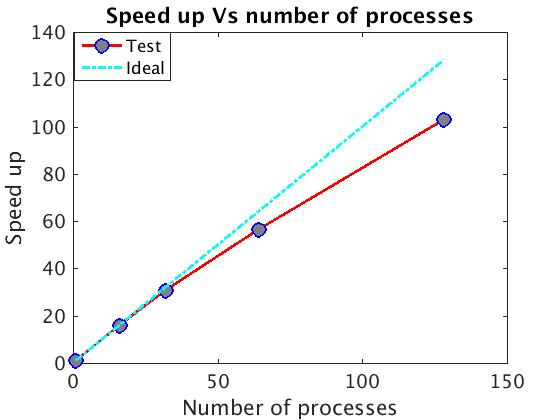
\includegraphics[scale=0.35]{strong}
\caption{Strong scalability test results}
\label{fig:strong_scale}
\end{figure}

\begin{figure}[!t]
\centering
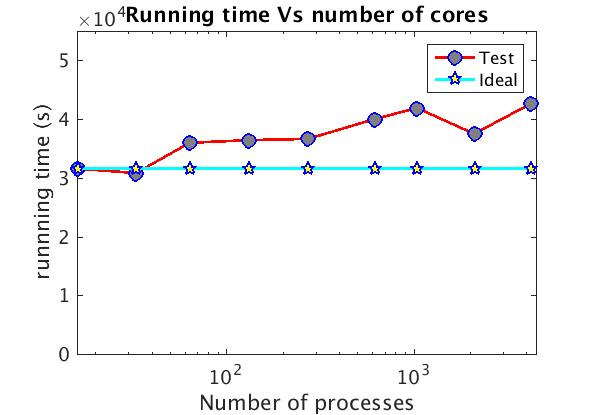
\includegraphics[scale=0.35]{weak_scale}
\caption{Weak scalability test results}
\label{fig:weak_scale}
\end{figure}

\begin{figure}[!t]
\centering
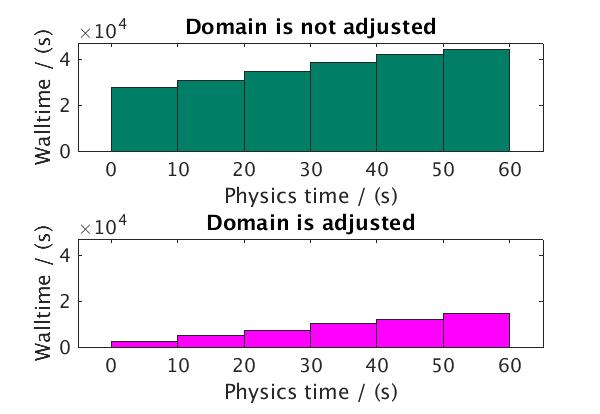
\includegraphics[scale=0.35]{adj_vs_no}
\caption{The effect of domain adjusting on simulation time. The figure on the top shows simultion time without domain adjusting, the figure on the bottom shows simultion time with domain adjusting. Different bins represent simulation time up to specific physics time indicated by $x$ axis.}
\label{fig:adj_vs_no}
\end{figure}
Experiments have been carried out on the computational cluster of Center for Computational Research (CCR) at Buffalo. E5645 CPUs running at 2.40GHz clock rate with 4GB memory per core on a Q-Logic Infiniband is used in these tests. Each node comprise of two sockets with 6 of these cores. Memory and level 3 cache are shared on each node. 
The initial domain is $[-4.8km,4.8km]\times [-4.8km,4.8km] \times [0km, 6km]$. Almost linear speed up is observed in figure \ref{fig:strong_scale}.
The weak scalability test is conducted with the same initial domain and various smoothing lengths. Each simulation is run for 400 steps. The average number of real particles of each process is kept constant at $25900$. As shown in figure \ref{fig:weak_scale}, simulation times increase around $1/3$ when number of cores increase from 16 to 4208. For the test problem in this paper, the volcanic plume will finally reach to a region of $[-30km \,\,\, 30km] \times [-30km\,\,\,30km] \times [1.5km\,\,\,40km]$ after around 400 seconds of eruption. When numerical simulation goes up to 90 seconds, the plume is still within a region of $[-10km\,\,\,10km] \times [-10km\,\,\,10km] \times [0km\,\,\,25km]$. This implies that adjusting of domain can avoid computing large number of uninfluenced air particles, especially for the beginning stage of simulation. Figure (\ref{fig:adj_vs_no}) shows that simulation time of the test problem is greatly reduced when we adopt the domain adjusting strategy in our code. 
%show a figure for initial pressure boundary condition
%shouw a figure for pressure boundary condition after several time steps.
\section{Verification and validation} \label{sec:verification-validation}
We will now present a series of numerical simulations that were used to verify and validate the model. The SPH plume model is first verified by a JPUE simulation. Velocity and mass fraction distribution both along the central axis and cross transverse are compared with experimental results. The parten of  ambient particles entrainment is also clearly shown. Then a simulation of representative strong volcano plume is conducted. Both global variables and local variable are comparable with simulation results from exisitng 1D and 3D plume models. Analysis on evolution of plume shows detailed air entrainment mechanism and the structure of plume are consistent with simulation results of existing 3D models. 
\subsection{Simulation of JPUE}
JPUE can be considered as a simplified volcanic plume. While the effect of stratified atmosphere and the effect of expansion due to high temperature in volcanic plume are not represented, JPUE reproduces the entrainment due to turbulent mixing which is one of the key elements in volcanic plume development. In this section, we will verify that our code and the turbulence model we adopted is able to reproduce feature of turbulent entrainment.
There exist consistently good experimental data \cite{papanicolaou1988investigations, list1982turbulent, dimotakis1983structure} that describe the JPUE flow field giving an insight into detailes of JPUE, such as transverse velocity and concetration profile.
% jet width along jet axis. 
As many of these experiments were conducted with liquid, we replace the original equation of state (equation(\ref{eq:EOS})) with a weakly compressible Tait equation of state \cite{becker2007weakly} to avoid solving the Poisson equation.
\begin{equation}
p=B[(\dfrac{\rho}{\rho_0})^{\gamma}-1]
\end{equation}
with $\gamma=7$ and $B$ is evaluated by:
\begin{equation}
B=\dfrac{\rho_0 c^2}{\gamma}
\end{equation}
Where $c$ is speed of sound in the liquid. Energy equation is actually decoupled from momentum and mass conservation equation by using this EOS. In addition, the "atmosphere" is assumed to be uniform and gravity is set to be zero in JPUE simulation. We set the temperature and density of ejected material from the vent the same as its surrounding ambient. This will further simplify the scenario for the convenience of studying turbulent mixing.
In this section, an axisymmetric JPUE which ejects from a round vent is simulated. The concetration and velocity distribution in both axial and radial direction were compared against various available experimental results.
\begin{figure}
\hfill
\subfigure[Velocity]{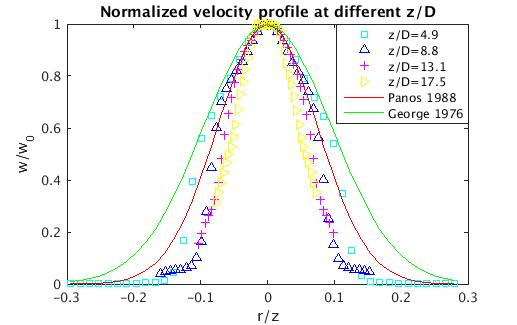
\includegraphics[width=5cm]{vel_cross}}
\hfill
\subfigure[Concetration]{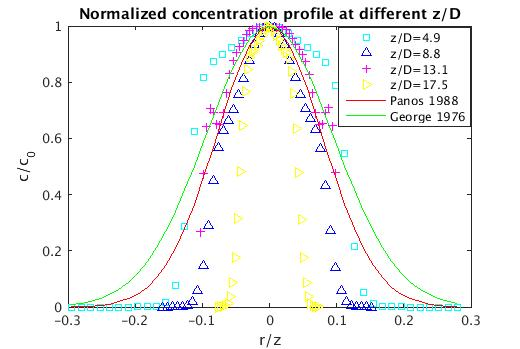
\includegraphics[width=5cm]{conc_cross}}
\hfill
\caption{Dimensionless concetration and velocity distribution across the cross-section.}
\label{fig:JPUE_cross-section}
\end{figure}

\begin{figure}
\hfill
\subfigure[Velocity]{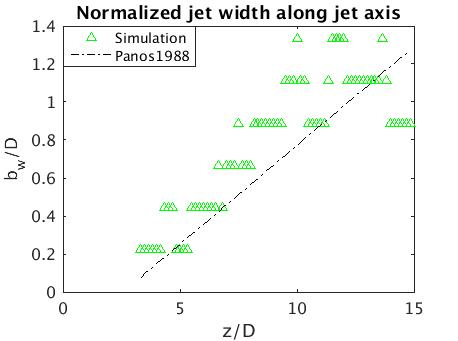
\includegraphics[width=5cm, height=4cm]{velo_along_axis}}
\hfill
\subfigure[Concetration]{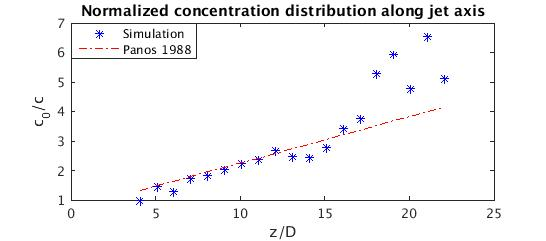
\includegraphics[width=5cm, height=4cm]{conc_along_axis}}
\hfill
\caption{Dimensionless concetration and velocity distribution along centraline.}
\label{fig:JPUE_along-axis}
\end{figure}
One overall feature of JPUE is "self-similarity" which means that the evolution of the JPUE is determined soley by the local scale of length and velocity which theoretically account for the fact that the rate of entrainment at the edge of JPUE is proportional to a characteristic velociy at each height. As a results, physical and numerical experiments with different setups are comparable on a non-dimensional basis. A three dimensional JPUE simulation is coducted and results are compared with experiments \cite{papanicolaou1988investigations, george1977turbulence} for verification purpose in figure \ref{fig:JPUE_cross-section} and figure \ref{fig:JPUE_along-axis}. Experimental data of concentration and velocity distribution across the cross-section was fit into a Gaussian profile: $\dfrac{\varphi}{\varphi_c}=exp[-coef (\dfrac{r}{z})^2)]$ (solid line) even though there is no priori reason. Panos also fit concentration distribution and jet width based on velocity along central line into a straight line : $\dfrac{\varphi_0}{\varphi_c}=slope (\dfrac{z}{D} + intercept)$ (dash line). Where $\varphi$ is either velocity or concetration, the subscript $c$ represents the centraline, $0$ represents the cross-sectionally averaged exit value. $r$ is the distance from the centraline on any cross-section. $z$ is the axial distance from the origin of the jet transverse section underconsideration. $D$ is the diameter of vent. The coefficient $coef$ for concetration is 80 and 50 respectively according to Panos and George. $coef$ for velocity is 90 and 55 respectively according to Panos and George. 
$slope$ for jet width based on velocity is 0.104 and for concetration is 0.157. $intercept$ for jet width based on velocity is 2.58 while that for the concetration is 4.35.\\
%$slope$ for velocity is 0.149 and for concetration is 0.157. $intercept$ for velocity is 2.56 while that for the concetration is 4.35.\\
%I also need to compare the velocity and concentration at z/d=40
Although both velocity and concetration are found to be well matched with experimental results, a small disparity in both velocity and concetration are observed near the boundary of the jet. There are several factors that would attribute to such disparity. Reynolds number are not reported in many experiments assuming a high enough Reynolds number. In addition, some details of the of the experiments, such as exit velocity profile, viscosity of the experimental liquid, are not reported, neither. These factors prevent us from repeating these experiments exactly with simulation. However, the features of JPUE is correctly reproduced with our code.\\
We also investigated the mixing due to turbulence in JPUE simulation by checking the mixture of two phases: the ejected liquid and ambient liquid. What need to be noticed is that the mass of particle of phase one (blue) is 8 time of that of phase 2. It is a trade off between resolution and computational expense to give particle of two phases different particles mass. Both advanced SPH techniques like adaptive particles size and better data management and access strategies need to be exploited to address this issue. It is shown in figure \ref{fig:Turb_mixing} that the ejected material and ambient fluids are mixed through eddies at the outer shear region. And the inner dense core dispersed gradually due to erosion of the outer shear region. Hence, our confidence in the numerical correctness of this model is greatly reinforced.
\begin{figure}
\hfill
\subfigure[mass fraction of erupted material]{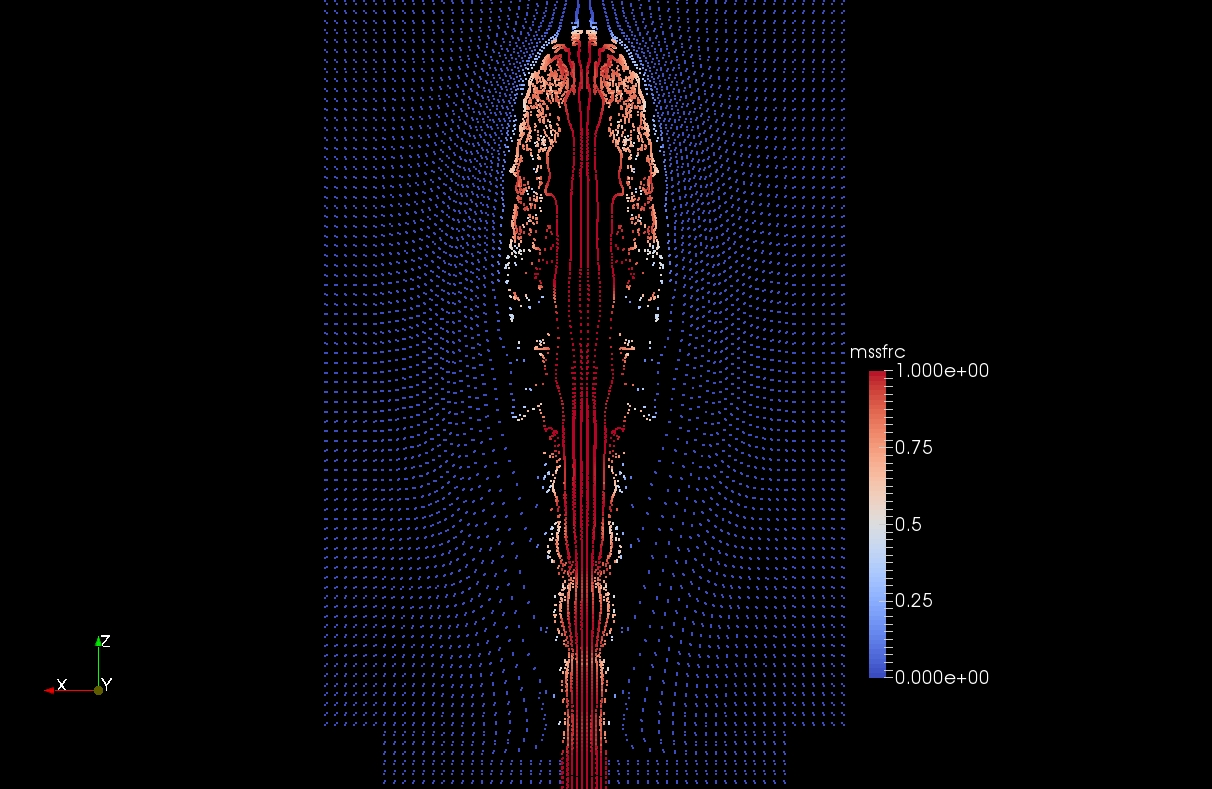
\includegraphics[width=5cm]{turb_mix_mssfrc}}
\hfill
\subfigure[entrainment of air particles]{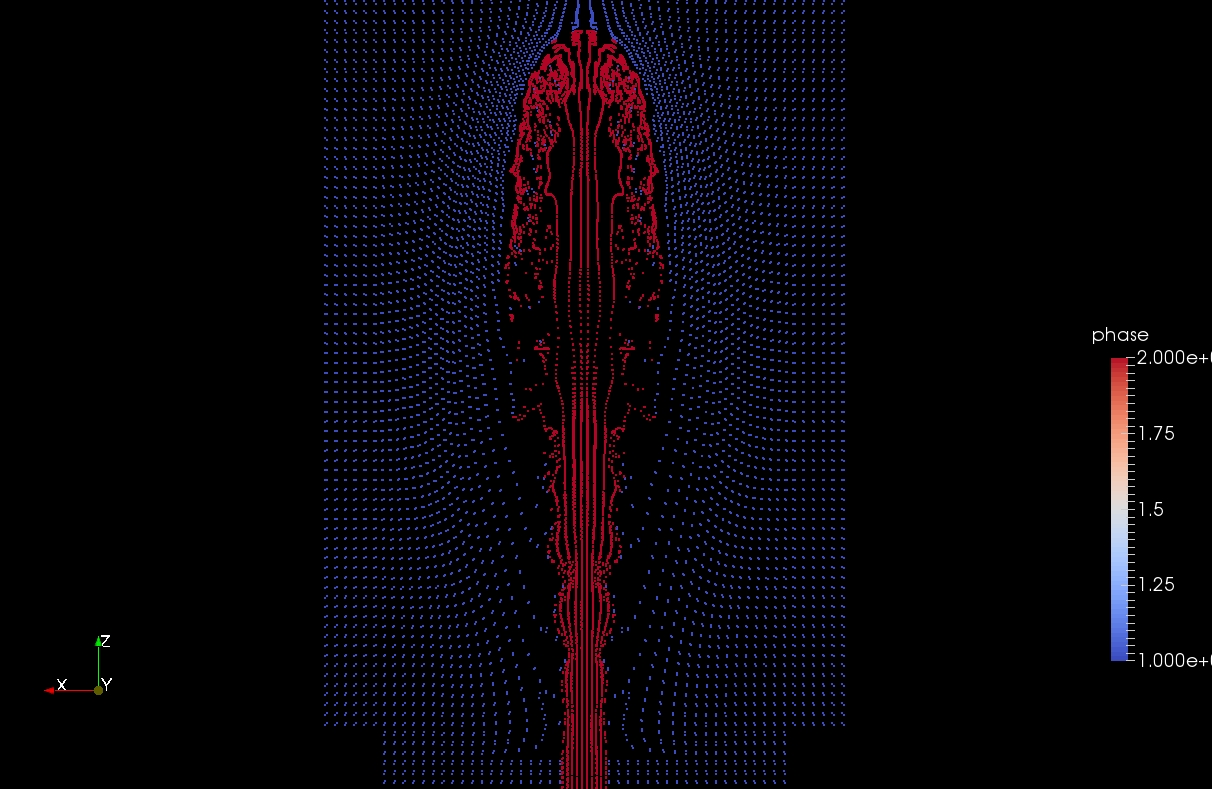
\includegraphics[width=5cm]{turb_mix_phase}}
\hfill
\caption{First figure shows the mass fraction of erupted material.The second figure shows particle distribution at the moment corresponding to first figure. Ambient particles (blue) are gradually entrained and mixed with erupted particles (red) as jet flows upward.}
\label{fig:Turb_mixing}
\end{figure}

\subsection{Simulation on Plume}
The physics of volcano plume is more complicated than JPUE in several aspects. Besides turbulent entrainment of ambient fluids, development of volcano plume also involves heating up of entrained air and then expanding in a stratified atmosphere. We will aplly our model to simulate plume development and in purpose of further validation. A strong eruption column without wind is tested in this section. Input parameters, material properties and atmosphere are choosen to be the same as one case in an inter-comparison study on eruptive column models \cite{costa2016results}. The strong plume scenario was based on climactic phase of the Pinatubo eruption(Philippines, 15 June 1991). Material properties are selected based on properties of Pinatubo and Shinmoe-dake eruption.The plume evolution process are first investigated. Then both global variable and local variables are compared with existing models. 
%Finally the sensitivity of plume development on input parameters is studied.
\subsubsection{Evolution of plume} 
\begin{figure}
\center
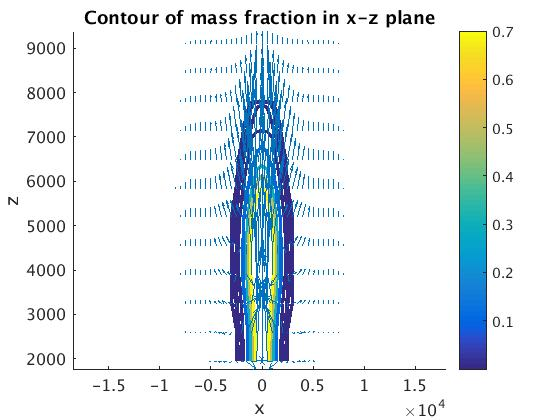
\includegraphics[width=5cm]{t15}
\caption{Contour of mass fraction and velocity at 15 seconds, column rises up quickly due to intial momentum.}
\label{fig:strong_t15}
\end{figure}

\begin{figure}
\center
{
\hfill
\subfigure[Overall view ]{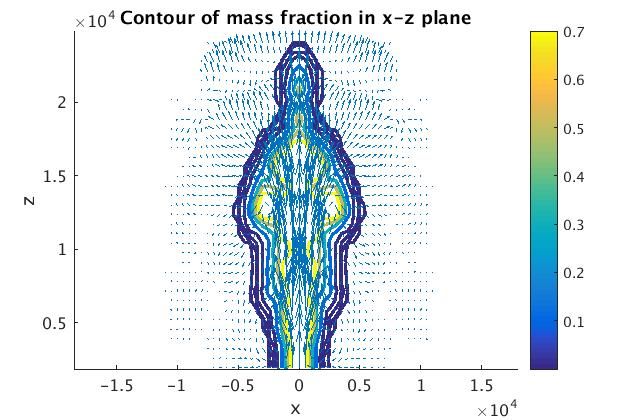
\includegraphics[width=5cm]{t50}}
\hfill
\subfigure[Detailed view]{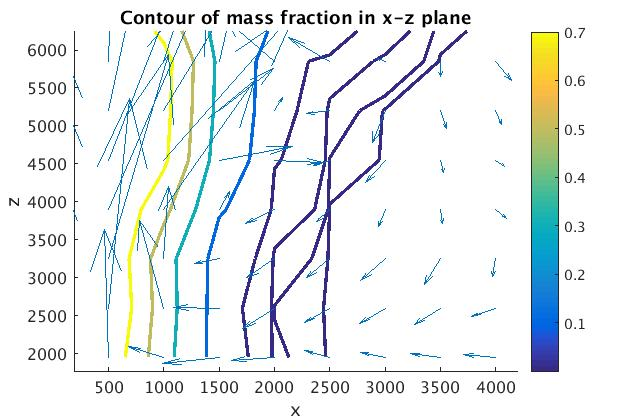
\includegraphics[width=5cm]{t50_local}}
\caption{Contour of mass fraction and velocity at 50 seconds, column keeps rising up and at the same time entraining air into the plume at the outer shear region. The entrainment of air is shown in detailed view where velocity distribution is more clear}
\label{fig:strong_plume_t50}
}
\end{figure}

\begin{figure}
\center
{
\hfill
\subfigure[Overall view ]{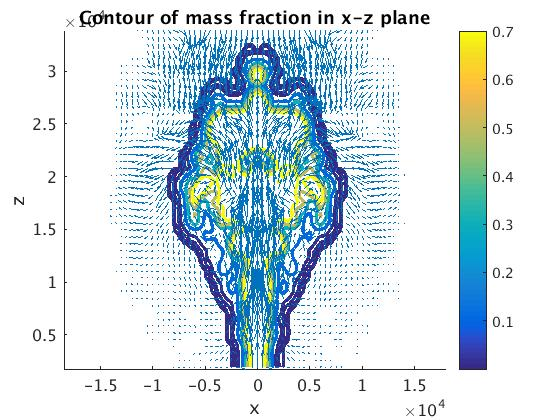
\includegraphics[width=5cm]{t100}}
\hfill
\subfigure[Detailed view]{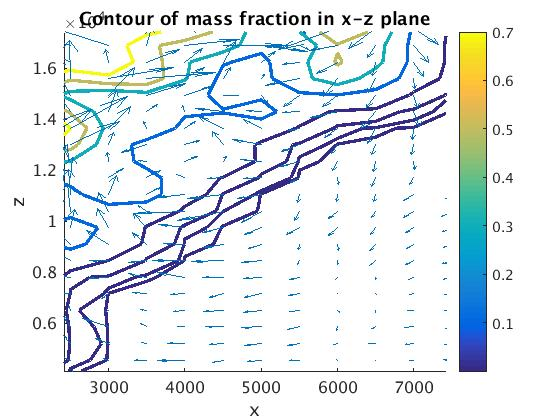
\includegraphics[width=5cm]{t100_local}}
\caption{Contour of mass fraction and velocity at 100 seconds, it keeps rising up and entraining air. The entrainment of air is shown in detailed view where velocity distribution is more clear}
\label{fig:strong_plume_t100}
}
\end{figure}

\begin{figure}
\center
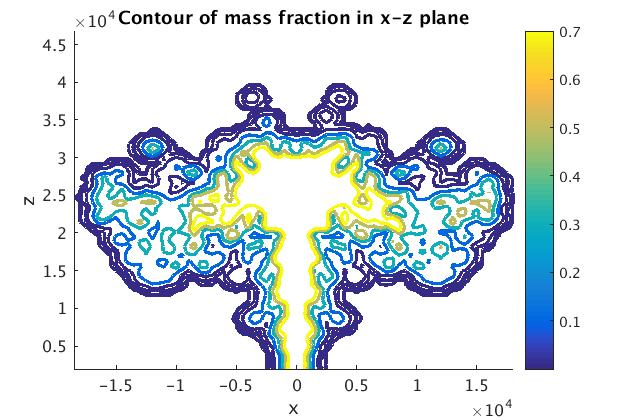
\includegraphics[width=5cm]{t200}
\caption{Contour of mass fraction at 200 seconds, plume reaches its top height}
\label{fig:strong_t200}
\end{figure}

\begin{figure}
\center
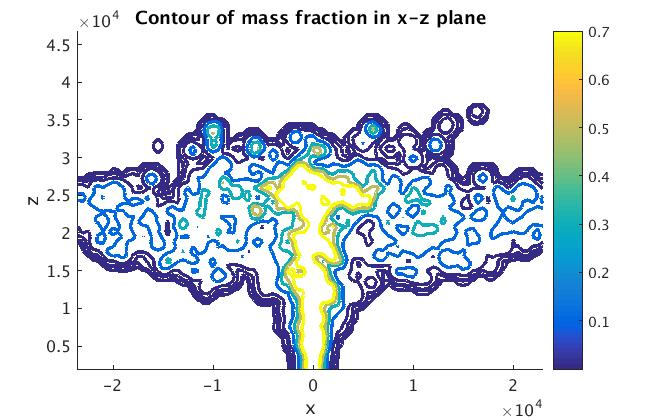
\includegraphics[width=5cm]{t300}
\caption{Contour of mass fraction at 300 seconds, the cloud is spreading}
\label{fig:strong_t300}
\end{figure}

Figure \ref{fig:strong_t15}~\ref{fig:strong_t300} shows the dynamic evolution process of volcano plume. The contour level of mass fraction are 0.7, 0.5, 0.3, 0.1, $1\times 10 ^{-1}$, $1\times 10 ^{-2}$, $1\times 10 ^{-3}$, $1\times 10^{-4}$ and $1\times 10^{-5}$. The plume keeps rising up and entraining air into the plume untill it reaches its top height(around t=200 seconds). The mixtures of erupted material and air falls back to neutral height and starts spreading radially after reaching the top height. Detailed velocity quiver plots show eddies at the edge of column entrainning air into the plume. It also shows in these figures that the plume near the vent maintains a concentric structure with an inner dense core surrounded by an outer shear region which is consistent with observation and previous simulation and observations.
\subsubsection{Global and local variables}
One of the key global quantities of great interest is the altitude to which the plume rises. The top height predicted by our model is around 40km which agrees well with other plume models. For example, the height predicted by PDAC is 42500m, by SK-3D is 39920m, by ATHAM is 33392m. As for local variables, the temperature, the mass fraction of entrained air, the gas mass fraction, the mass fraction of solid, the radius of the plume as a function of height are compared with existing 1D and 3D models in figure \ref{fig:strong_local_radius}-\ref{fig:strong_local_temp}. 
%Velocity and density show general agreement in shape of the profile with exising 3D and 1D models.
\\
\begin{figure}
\center
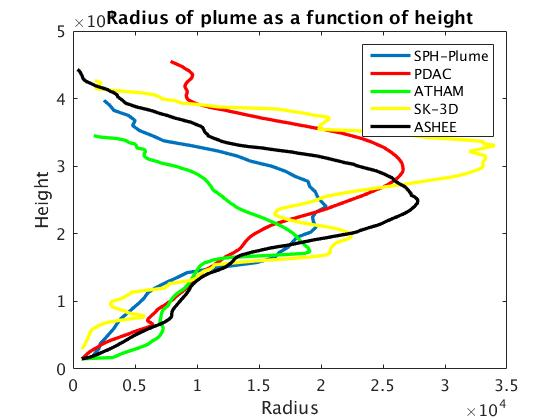
\includegraphics[width=5cm]{radius_strong}
\caption{Radius of the strong plume without wind after reaching its top height}
\label{fig:strong_local_radius}
\end{figure}
The profile of plume radius matches with simulation results of exisitng 3D models in general sense. The basic phenomena in volcano plume development is correctly captured by our model: the plume first rises up to its top height and then falls down to the netural buoyancy height and starts expanding.\\
\begin{figure}
\hfill
\subfigure[The mass fraction of air entrained into the plume ]{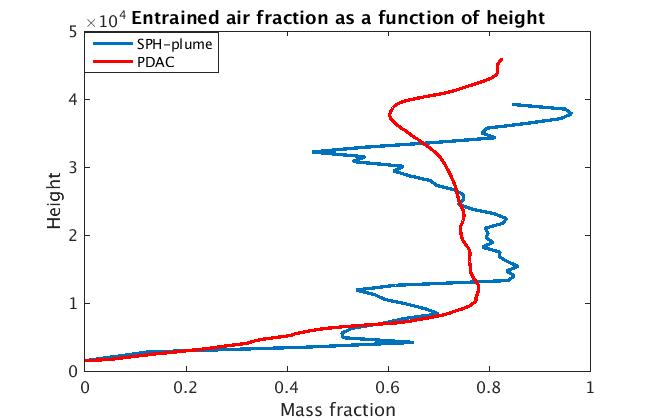
\includegraphics[width=5cm]{entrained_air}}
\hfill
\subfigure[The mass fraction of gas (air+vapor) in the plume ]{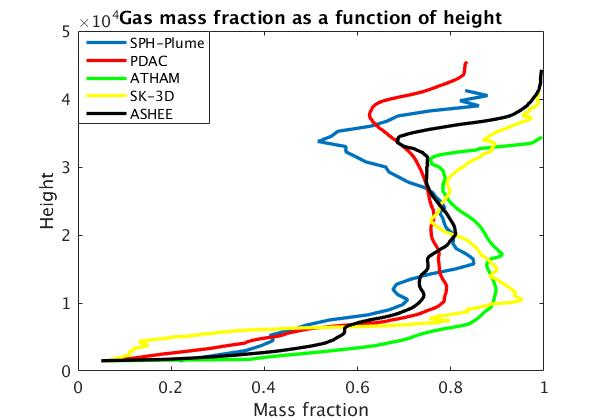
\includegraphics[width=5cm]{gas_frac}}
\hfill
\subfigure[The mass fraction of solid in the plume ]{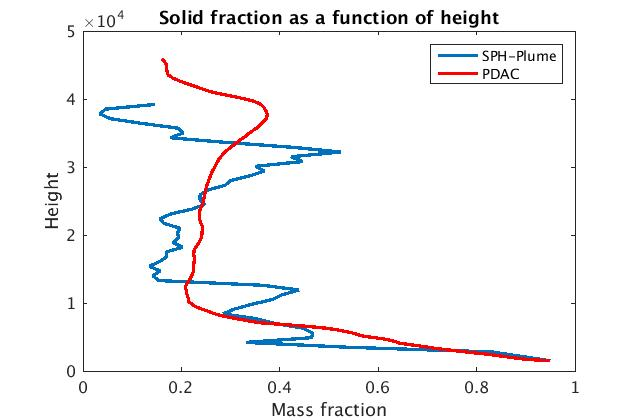
\includegraphics[width=5cm]{solid_frac}}
\hfill
\caption{The mass fraction of entrained air, gas, and solid as a function of height}
\label{fig:strong_plume_mass_fraction}
\end{figure}
As the height increase, the amount of entrained air will increase. At the netural height, where the umbrella expanding, the entrainment decrease due to lack of air surrounding the column. The profile of mass fraction of gas, solid and air are consistent with these results predicted by exisitng 3D plume models in general.
\begin{figure}
\center
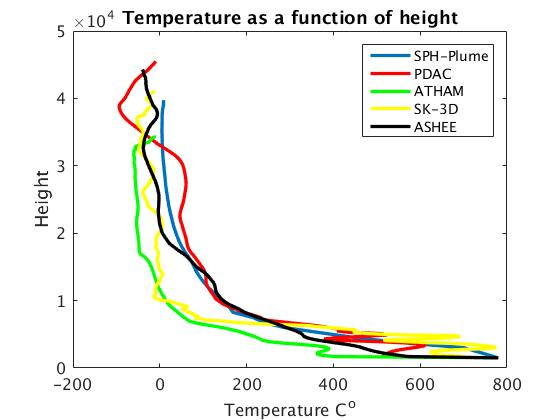
\includegraphics[width=5cm]{Temp}
\caption{Temperature as a function of height}
\label{fig:strong_local_temp}
\end{figure}
More and more cool air will be entrained into the plume and mix with hot erupted material as the plume rises up. Heat exchange between air and erupted material will also cool the plume down. So the temperature of the plume decreases as the height increase as shown in figure \ref{fig:strong_local_temp}. 
%However, a big disparity in density profile were observed originally. Several factors attribute to this disparity. The first one is normalization process (equation \ref{eq:CSP-function-approximation-1d}) which was originally proposed for single phase flow. Second, we are using a constant smoothing length for both phases, which is larger than usual value for phase two who bears smaller mass and  is smaller than usual value for phase one who bears larger mass. Relative larger smoothing length will smooth out large density to a smaller value. Variable smoothing length method which might mitigate this issue is avoid due to its high computational cost. 
%\subsubsection{Parameter sensitivity}
To summarize, analysis on JPUE simulation verified the correctness of the code. The comparison with existing 3D models further verified the correctness of our code. The dynamic evolution of the plume agrees with mechanism analysis of plume development, which convinced us that the physics model that takes major factors in plume development into accout.
\section{Conclusion and discussion} \label{sec:conclusion}
A new plume model was developed based on SPH method. Advanced numerical  techniques in SPH were exploited and talored for this model. High performance computing was used to mitigate confliction between accuracy (depends on comprehensiveness of the model, resolution, order of accuracy of numerical methods, shceme for time upgrading ...) and simulation time (depends on, comprehensiveness, resolution, order of accuracy of numerical methods, shceme for time upgrading ... and computational techniques). The correctness of the code and model was verified and validated by a series of test simulation.\\
Currently existing 3D models focus on certain aspect of the volcano plume (PDAC on pyroclastic flow, ATHAM on microphysics, and SK-3D on entrainment with higher accuracy and higer oder of accuracy) and hence, naturely, different assumptions were made in these models. However, these different aspects of volcano plume are not independent and actually are coupled. In addtion, there is no absolute boundary to determine which kind of hazard is dominant in certain eruption. So it is necessary to simulate all associated hazards in one model. Actually, effort has already been put on developing more comprehensive plume models. For example, a large-particle module (LPM) was added to ATHAM to track the paths of rocky particles (pyroclasts or tephra) within the plume and predicts where these particles fall\citep{kobs2009modeling}. We were motivated by such a tendency of plume modeling to choose SPH as our numerical tool. As mentioned in the previous section, SPH method has very good extension features and adding of new physics requires tiny modification on the code compared with mesh-based methods. The last but not the least, the dramatisc development of computational power makes establishing of a comprehensvie model feasible. Even though right now, current computational capacity does not allow us to have too comprehensive model, the easy-extension feature of SPH makes it feasible to keep adding new physics into the model when necessary. What presented in this paper is actually our initial effort and results towards developing a first priciple based plume model with comprehensive physics, adopting proper numerical tools and power of high performance computing. More advanced numerical techiques, such as adaptive particle size, Godnuv-SPH, semi-explicit time advancing scheme and better data management strategies and algorithms are on our list to exploit.
\bibliographystyle{plainnat}
\bibliography{Reference}
\end{document}